\chapter{Operando EPR Spectroscopy of TEMPO-Salen Electrochemical Cells}

\section{Electron Paramagnetic Resonance}
In this section, the phenomenon of electron paramagnetic resonance is briefly described with details that are required to interpret the spectra of a charging electrochemical cell containing nitroxide radicals attached to a conjugated polymer backbone. After the introduction of the spin Hamiltonian, an experimental procedure to observe the corresponding spin transitions with continuous microwaves is described. The characteristic spectra of nitroxide radicals in various environments are described. That information is used to decompose the complex spectra of a charging cell to identify the state of charge of the cell and the by-products that are being released during the cell operation.

\subsection{The Spin Hamiltonian}
\paragraph*{Electron Spin}
In the Poincaré group of special relativity~\cite{poincare_1905}, when rotations are considered together with the relativistic boosts~\cite{einstein_s_rel}, there emerges an additional quantity that is associated with rotation and is preserved together with the orbital angular momentum, yet this quantity is retained for point objects - it is called spin~\cite{kuprov_2023}. Spin is quantized~\cite{SternGerlach1922}; it can take values in integer- or half-integer multiples of the Planck's quantum of action $\hbar$ up to a certain magnitude $S$. The electron, as a fundamental particle and a fermion, bears a half-integer spin with a magnitude of $S=1/2$. 

\par
An isolated electron has two degenerate spin states - spin-up $\vert{\uparrow}\rangle$ and spin-down $\vert{\downarrow}\rangle$ - that are eigenfunctions of the square of the spin operator $\hat{s}^2$ with the same (degenerate) eigenvalue $\hat{s}^2\vert{\uparrow}\rangle=\hat{s}^2\vert{\downarrow}\rangle=\frac{3}{4}\hbar^2$. The states $\vert{\uparrow}\rangle$ and $\vert{\downarrow}\rangle$ are also eigenfunctions of the $z$ component of the spin operator, but correspond to different (non-degenerate) eigenvalues $m_s=\pm\hbar/2$~\cite{Sakurai}: 

\begin{equation}
\label{eq:sz_states}
\hat{s}_Z\vert{\uparrow}\rangle = +\frac{\hbar}{2}\vert{\uparrow\rangle}
\end{equation}
\begin{equation*}
\hat{s}_Z\vert{\downarrow\rangle}=-\frac{\hbar}{2}\vert{\downarrow\rangle}
\end{equation*}


\paragraph*{$\textbf{g}$ factor}

Spin combines with the charge of the electron to endow the electron with a magnetic moment $\mu_{spin} = \gamma S$, where $\gamma=\frac{g_e\mu_B}{\hbar}\approx 28$~GHz/T is the gyromagnetic ratio of the electron, $\mu_B=\hbar e/m_e$ is the Bohr magneton and $g_e \approx 2$ is the electron $g$ factor~\cite{Carrington_g_factor}. The $g$ factor connects the spin of a particle with a magnetic moment that the particle expresses through interactions with external fields~\cite{Schwinger1948}. The Dirac quantum theory of the electron predicts $g_e=2$~\cite{dirac1928}. However, up to date, $g_e = 2.00231930436256(35)$ has been measured to the unprecedented accuracy of 0.13~ppt~\cite{Fan2023_PRL}. This measurement lies at the frontier of modern particle physics and the accordance of the measured $g_e$ with the value obtained with quantum electrodynamics~\cite{Schwinger1948,Fan2023_PRL} is the triumph of the quantum field theory~\cite{Feynman_1949}. 
\par
Depending on the local environment of an electron, its $g$ factor can change from $g_e$ due to the spin-orbit coupling that changes the observed magnetic moment of the electron~\cite{Carrington_g_factor}. The magnetic moment of an electron can therefore be used as an extremely sensitive probe of the electron's local environment. The $g$ factor of an electron localized in a molecular orbital can be anisotropic, depending on the shape of the orbital. Anisotropic $g$ factor is represented by a $3\times3$ $\textbf{g}$ matrix that can almost always be diagonalized~\cite{Carrington_g_factor} by an appropriate rotation of the molecular coordinate system.



\paragraph*{Zeeman Splitting}

When an electron is placed in a static magnetic field $\vec{B_0}=B_0 \vec{e_z}$, its magnetic moment experiences a torque and precesses in the $xy$ plane about the field axis with the Larmor frequency $\omega_L = \gamma B_0$. The magnetic moment of the electron has two possible projections on the magnetic field axis, according to \ref{eq:sz_states}. The two corresponding eigenvalues $\pm\frac{\hbar}{2}$ define the energy difference between the states $\vert{\uparrow\rangle}$ and $\vert{\downarrow\rangle}$ when the spin couples to the external magnetic field, that is known as the Zeeman splitting. The energy difference between $\vert{\downarrow}\rangle$ and $\vert{\uparrow}\rangle$ in a magnetic field is the Zeeman energy. 

\par

The energy of an isolated electron placed in the external magnetic field $\vec{B_0}$ is the energy of the electron's magnetic moment in that field, that is given by the eigenvalue of the spin Zeeman Hamiltonian: $\hat{H}_{EZ} = \frac{\mu_B}{\hbar} \vec{B}_0g_e\vec{\hat{s}}$. In the laboratory frame of reference $\vec{B_0}\parallel\vec{e_z}$, $\left[\hat{H}_{EZ},\hat{s}_z\right]=0$, so $\hat{H}_{EZ}$ and $\hat{s}_Z$ share the two eigenfunctions $\vert{\uparrow\rangle}$ and $\vert{\downarrow\rangle}$. The energies of the corresponding states are $E_{EZ}^{\pm} = \pm \frac{1}{2}\mu_B g B_0$ (see Figure~\ref{fig:cwerp_free_electron}), and their difference is the Zeeman splitting:

\begin{equation}
%\label{eq:epr_resonance_condition}
\label{eq:electron_zeeman}
\Delta E_{EZ} = \mu_B g_e B_0
\end{equation}

The measurement of the magnetic moment of an electron can be done by measuring its Zeeman energy. The local molecular environment affects the electron's magnetic moment through spin-orbit coupling which can be seen as a deviation in the electron's $g$ factor~\cite{Carrington_g_factor}.



\paragraph*{Nuclear Spin and Nuclear Zeeman Splitting}
A proton has a half-integer spin $S=1/2$ that results in a magnetic moment $\mu_p = \mu_e\frac{m_e}{m_p}$, that is $\frac{m_p}{m_e}\approx1836$ times smaller than the electron's magnetic moment. A neutron bears no charge but also has a half-integer spin $S=1/2$. An atomic nucleus that consists of protons and neutrons has a magnetic moment which is a vector sum of the aligned spins of its protons and neutrons. The spin of a nucleus is defined by the arrangement of its nucleons and by the nuclear charge. A nitrogen nucleus has 7 protons and 7 neutrons that total in a nuclear spin $I=1$ which, with the g factor for the nitrogen nucleus $g_N$, results in the nuclear magnetic moment of $\mu_N=\mu_B\frac{m_e}{m_N}g_NI$ that splits into three Zeeman levels corresponding to the three possible projections of the nuclear spin on the magnetic field axis, $m_I=-1,0,+1$, analogously to the electron with $m_S=1/2,-1/2$. The nuclear Zeeman splitting is more than two orders of magnitude weaker than the electron Zeeman splitting because of the difference in the masses of the particles.

\paragraph*{Hyperfine Interaction}
The magnetic moments of an electron and a magnetic nucleus, such as nitrogen, couple in the hyperfine interaction: $H_{HF}=\vec{\hat{s}}\textbf{A}\vec{\hat{I}}=H_F+H_{DD}$ with the hyperfine coupling tensor $\textbf{A}$. The isotropic part $H_F=a_{iso}\vec{\hat{s}}\vec{\hat{I}}$, or the Fermi contact interaction, scales with the probability density of the electron at the position of the nucleus $a_{iso}=\frac{2}{3}\frac{\mu_0}{\hbar}g_e\mu_eg_n\mu_n\vert\psi(0)\vert^2$~\cite{Schweiger2001_hfi}. The anisotropic part $H_{DD}=\vec{\hat{s}}\textbf{T}\vec{\hat{I}}$ with the dipolar coupling tensor $\textbf{T}$ takes into account the anisotropic magnetic dipole coupling between the magnetic moments of the electron and the nucleus. $\textbf{T}$ depends on the shape of the electron orbital, its $3\times3$ Cartesian matrix representation depends on the molecular frame of reference and can be diagonalized by rotating the coordinate system. The matrix representation of the hyperfine coupling tensor $\textbf{A}$ can be written in as the sum of its isotropic and anisotropic parts: $\textbf{A}=a_{iso}\mathds{1}_3 + \textbf{T}$~\cite{Weil_Bolton}. In its diagonal matrix representation $\textbf{A}$ reduces to its three principal components $[A_{xx}, A_{yy}, A_{zz}]$. The values of $\textbf{A}$ are typically given in MHz.

\paragraph*{Exchange Interaction}
In a system of closely placed electrons, such as in a film of densely packed radicals, the electron orbitals may overlap significantly and the radicals may exchange electrons. The energy required to exchange the electrons is called the exchange coupling $H_{exch} = \vec{\hat{s_1}}\textbf{J}\vec{\hat{s_2}}$, that becomes considerably large at inter-spin distances below $r<1.5$~nm or with a large spin delocalisation~\cite{Schweiger2001_exch}. The positive $\textbf{J}$ corresponds to a weak coupling between $s_1$ and $s_2$ which leads to an antiferromagnetic or antiparallel alignment of spins with a total $S=0$, whereas the negative $\textbf{J}$ causes the strong inter-spin coupling which leads to a ferromagnetic alignment with $S=1$~\cite{Schweiger2001_exch}.\\

MOVE this to EPR section!
The stochastic, gaussian random modulation theory
of exchange narrowing [ 1-33 predicts that the half-
width at half maximum intensity of a strongly ex-
change narrowed electron pararnagnetic resonance
(EPR) line is given by
(1)
\begin{equation}
\Delta B_0 \approx\frac{10}{3}\left(\frac{H_p^2}{H_e}\right)
\end{equation}

and the resonance lineshape is lorentzian.
Hz is the mean square dipolar field and He is an
effective exchange field which is proportional to the
mean exchange integrd J
\cite{Oreilly_1971}


%\paragraph*{Magnetic Dipole-Dipole Interaction}
%The dipole-dipole interaction between the two neighboring electron spins contributes one more term to the spin Hamiltonian: $H_{dd} = \vec{\hat{S_1}}\textbf{D}\vec{\hat{S_2}}$ that depends on the distance between the spins. 

\paragraph*{Nuclear Quadrupole Moment}
The nitrogen nucleus has a spin greater than 1/2 which alters the charge distribution within the nucleus which gives rise to a non-vanishing nuclear electrical quadrupole moment $Q$~\cite{Schweiger2001_exch}. The interaction between the asymmetrically distributed charge and the gradient of the electric field at the nucleus is given by the nuclear quadrupole Hamiltonian $H_{NQ}=\vec{\hat{I}}\textbf{P}\vec{\hat{I}}$ with the nuclear quadrupole tensor $\textbf{P}$ that describes the coupling of the nuclear quadrupole moment to the electric field gradient.

\paragraph*{The Spin Hamiltonian}
For the interactions considered in this thesis, the following Hamiltonian will be applied to describe the interactions of unpaired electron spins with their local environments, ranging by their magnitude:
\begin{equation}
H = H_{EZ} + H_{HF} + H_{J} + H_{NZ} + H_{NQ}
\end{equation}

The electron Zeeman term $H_{EZ}$ defines the requirements on the hardware and sets the range of the magnetic fields used in the spectroscopic experiments. The hyperfine interaction term $H_{HF}$ allows for reconstruction of the hyperfine coupling tensor from the recorded spectra which is used as a marker to identify the molecular structure and dynamics of the mobile molecular fragments that are released during the operation of an electrochemical cell. The exchange interaction term $H_{J}$ scales with the concentration of the electrons, so the information about $\textbf{J}$ can be used to characterize the packing of the molecular fragments in the electrode. The nuclear quadrupole interaction term may lead to spectral distortions in a highly charged cathode where electric fields may be sufficiently strong to introduce noticeable nuclear quadrupole couplings to the nitrogen nuclei.

\paragraph{Energy Diagram of the Spin Hamiltonian}


\subsection{cwEPR spectroscopy}
\label{subs:cwEPR_spectroscopy}
First observed in 1944~\cite{Zavoisky_1945_JP,zavoisky_1945,salikhov_2015}, the phenomenon of electron paramagnetic resonance had quickly become a tool for probing local molecular environments in species that contain unpaired electron spins. A free electron, that does not interact with its environment and has $g=g_e$, experiences a Zeeman splitting of $\Delta E = g \mu_B B_0$, that corresponds to the energy of a photon with a frequency of $\nu=\Delta E / h$. A microwave photon can drive a magnetic dipole transition between the Zeeman-split spin states - this is called electron paramagnetic resonance (EPR). An X band microwave photon (IEEE X band, $\nu=8-12$~GHz, $\lambda=2.5-3.8$~cm, Figure~\ref{fig:cwerp_free_electron},left) can drive the magnetic dipole transition between $\vert{\uparrow\rangle}$ and $\vert{\downarrow\rangle}$ at $B_0\approx0.3$~T. In a continuous-wave electron paramagnetic resonance (cwEPR) experiment, the microwave frequency and power is kept constant while $B_0$ is scanned and the microwave absorption is observed. EPR happens around the $B_0$ values given by the spin resonance condition:

\begin{equation}
\label{eq:epr_resonance_condition}
\mu_B g_e B_0 = h\nu
\end{equation}

\begin{figure}[h]
\center
	\includegraphics[width=1.0\textwidth]{../scripts/plots/Free_Electron_EPRcombo.pdf}
	\caption{Left: Zeeman splitting for the energies of the two states of an isolated electron spin in a static magnetic field computed with EasySpin~\cite{Easyspin}. Vertical line is the magnetic dipole transition driven by a $9.4$~GHz microwave photon. Right: Microwave absorption and its derivative as a function of the static magnetic field for an unpaired electron spin with a 5~mT Gaussian broadening to show the realistic shape of the cwEPR spectrum.}
	\label{fig:cwerp_free_electron}
\end{figure}


\par
When $B_0$ reaches the value that satisfies Eq.~\ref{eq:epr_resonance_condition}, the sample starts absorbing microwaves. The absorbed microwave power recorded as a function of $B_0$ is the cwEPR spectrum (Figure~\ref{fig:cwerp_free_electron}, right, dashed). By construction, cwEPR spectrometers typically record the derivative of the microwave absorption vs. $B_0$ (Figure~\ref{fig:cwerp_free_electron}, right, solid). Advanced spin resonance techniques methods that involve coherent spin dynamics and pulsed microwave fields are discussed in Chapter~\ref{ch:pulsed_epr}.

\paragraph{Line Broadening}
"EPR spectra do not consist of a discrete set of infinitely sharp lines. Lines are broadened by dynamic effects (relaxation, tumbling, chemical exchange) or static effects (orientational disorder, unresolved hyperfine splittings, distributions in magnetic properties such as g, A, and D values)."


\paragraph{cwEPR spectrometer}

A basic cwEPR spectrometer consists of a magnet, a microwave source, a resonator and a microwave detector. Figure~\ref{fig:cwerp_spectrometer} depicts those elements with more details, including the sample - an electrochemical cell that is placed inside the microwave resonator and its SoC controlled with an external potentiostat.

\begin{figure}[h]
\center
	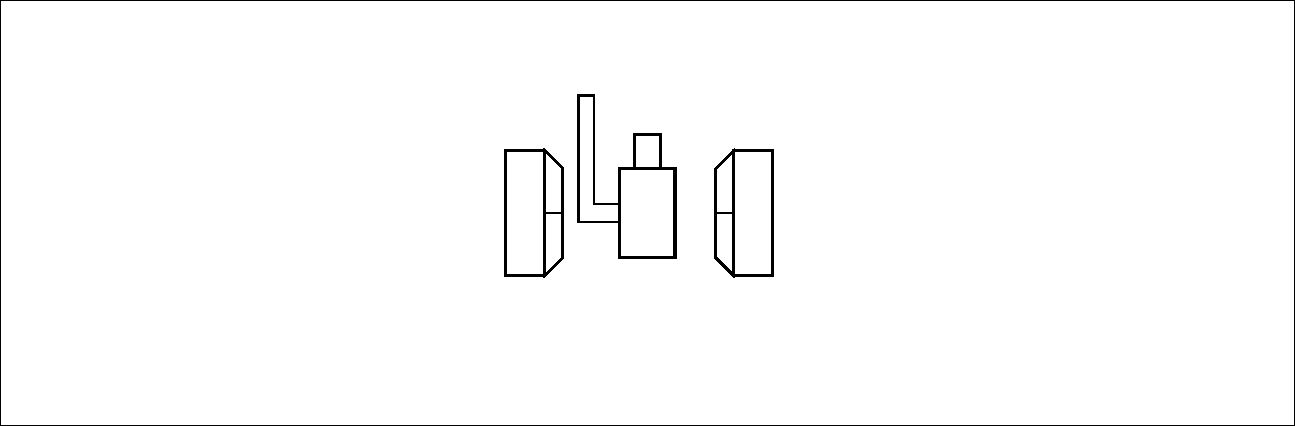
\includegraphics[width=0.9\textwidth]{./operando_epr/figures/cwEPR_spectrometer_diagram.pdf}
	\caption{Diagram of a cwEPR spectrometer}
	\label{fig:cwerp_spectrometer}
\end{figure}

\par
Continuous microwaves are generated with a klystron (MW source in Figure~\ref{fig:cwerp_spectrometer}) and directed towards the resonator (resonating cavity) through the signal arm that contains a variable attenuator and a circulator. The circulator directs the microwaves from the source to the cavity and passes the microwaves reflected from the cavity further to the microwave detector. The adjustable coupling iris between the circulator and the resonating cavity allows one to match the impedance of the cavity to the impedance of the signal arm so that minimal microwave power is reflected back from the cavity at a non-resonant field $B_0$. That impedance matching is called critical coupling. At the microwave detector, the microwaves reflected from the cavity are compensated by the microwaves with fixed microwave power and an adjustable phase, that pass through the reference arm. The signals from the two arms interfere destructively at the detector, so that there is no signal at the detector for non-resonant $B_0$.

\par
When the resonance condition (Eq.~\ref{eq:epr_resonance_condition}) is met, the incident microwaves are being absorbed by the sample and the resonator's $Q$ factor slightly changes. The change in the $Q$ factor decouples the resonator from the signal arm, that causes additional reflections in the signal arm. The microwaves in the signal arm that are not compensated by the reference arm become detected by the microwave detector - a biased semiconductor diode that has a linearly changing conductivity in the range corresponding to the incident microwave power. A phase sensitive detection with shallow modulation of $B_0$ increases the signal-to-noise ratio (SNR) and yields the derivative of the microwave absorption profile vs. $B_0$. The typically high $Q\gg1$ factor of the resonator further increases the SNR, as the decoupling of a resonator with higher $Q$ leads to a larger reflected microwave power.

\par
To ensure that only the magnetic component of the microwave is interacting with the sample, a standing microwave is formed in the resonating cavity. In the center of the cavity, the magnetic component of the microwave is maximized and the electric component is quenched. When a small sample is inserted in the center of the cavity, it is mostly the magnetic component of the microwave that is interacting with it. That allows one to drive magnetic dipole transitions without heating up the sample by the electric component. For larger samples as, for example, working electrochemical cells, the separation between the electric and magnetic microwave components does not hold within the full sample volume. Furthermore, the insertion of a cell containing metal electrodes and polar electrolyte into a resonator changes the distribution of the microwave field in it and lead to a non-resonant microwave absorption.


\section{cwEPR Spectroscopy of TEMPO Containing Molecular Fragments}
% todo: the reader knows about TEMPO, dits and ditbus. Show how they behave in cwEPR spectrometer.
% picture of molecule - spectrum - diagram
The stable TEMPO$^\bullet$ radical is widely used in the EPR spectroscopy as a spin probe and particularly in the EPR studies of TEMPO containing ORB materials~\cite{nakahara2002_cpl, nishide2004_electact, bahaceci2013_jpowersources, aydin2015_jsoistatelect, khodeir2019_softmatter, Zhang2018}. The spin density at the TEMPO$^\bullet$ radical is localized within the N-O bond~\cite{Owenius2001} and partially resides on the $I=1$ $^{14}$N nucleus, so to describe the EPR spectrum of an isolated TEMPO$^\bullet$ one has to take into consideration the electron Zeeman term $H_{EZ}$, the nuclear Zeeman term $H_{NZ}$ and the hyperfine coupling term $H_{HF}$. The unpaired electron spin on TEMPO$^\bullet$ has anisotropic g value, because of the asymmetry of its molecular orbital, so the $\textbf{g}$ matrix and the $\textbf{A}$ hyperfine coupling tensor are both anisotropic. $\textbf{g}$ is diagonal in the molecular frame of reference shown in Figure~\ref{fig:TEMPO_dft}. Its principal values are $\left[g_{xx}=2.009,g_{yy}=2.006,g_{zz}=2.002\right]$~\cite{Liu_2008,Bordignon2017}. The principal values of $\textbf{A}$ in the same frame are $\left[A_{xx}=20,A_{yy}=20,A_{zz}=100\right]$~MHz~\cite{Liu_2008,Bordignon2017}.

\subsection{Room Temperature Spectra of TEMPO$^{\bullet}$ Solutions}
Solution spectra of radicals are showing averaged values of $g$ and $A$ because of the fast molecular tumbling~\cite{Liu_2008,Carrington_solution_epr}. The observed $g$ value for a tumbling TEMPO$^{\bullet}$ is the average of the principal values of the $\textbf{g}$ matrix: $g = 1/3\left(g_{xx}+g_{yy}+g_{zz}\right)$. The anisotropic part of the hyperfine coupling tensor for the tumbling TEMPO$^{\bullet}$ also averages to zero, so only the isotropic hyperfine constant $a_{iso}$ determines the observed hyperfine coupling. CwEPR spectra of a 0.1~mM solution of TEMPOL measured at room temperature are shown in Figure~\ref{fig:cwEPR_monoTEMPO_diTEMPO}. The spectral simulation performed with EasySpin~\cite{Easyspin} yields $g=2.0055$ and $a_{iso}=43.8$~MHz.

\begin{figure}[h]
\center
	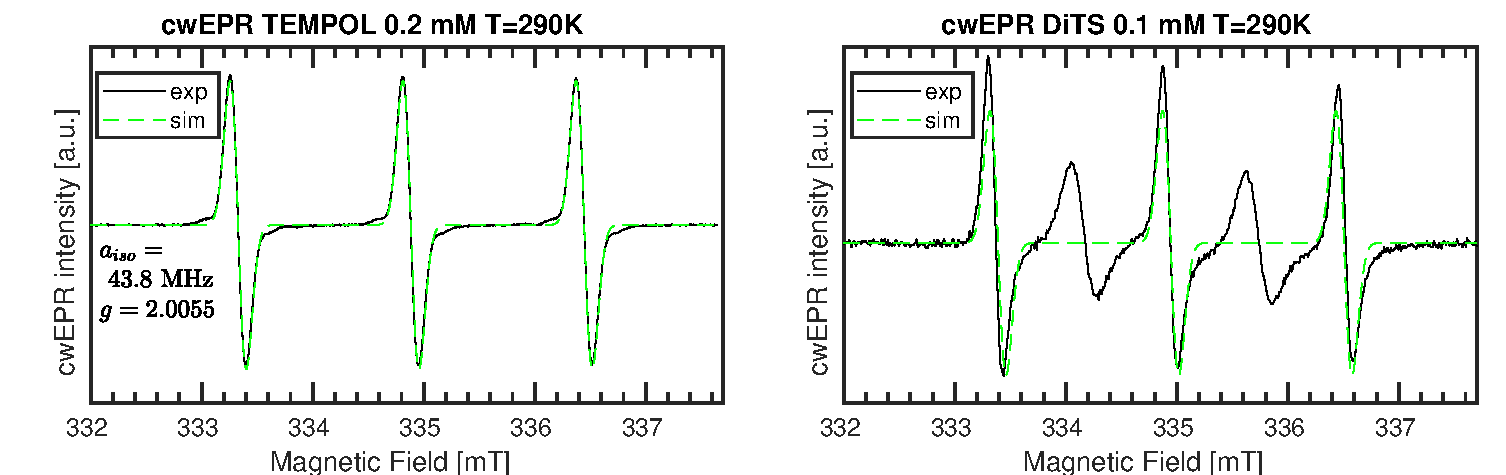
\includegraphics[width=1\textwidth]{./operando_epr/figures/TEMPOL/cwEPR_TEMPOL_vs_DiTS_RT.pdf}
	\caption{Room temperature cwEPR spectra of a low-concentration solutions containing mono- and di-TEMPO molecular fragments. Left: TEMPOL, Right: Di-Tempo-Salen.}
	\label{fig:cwEPR_monoTEMPO_diTEMPO_SOLUTION}
\end{figure}
\begin{figure}[h]
\center
	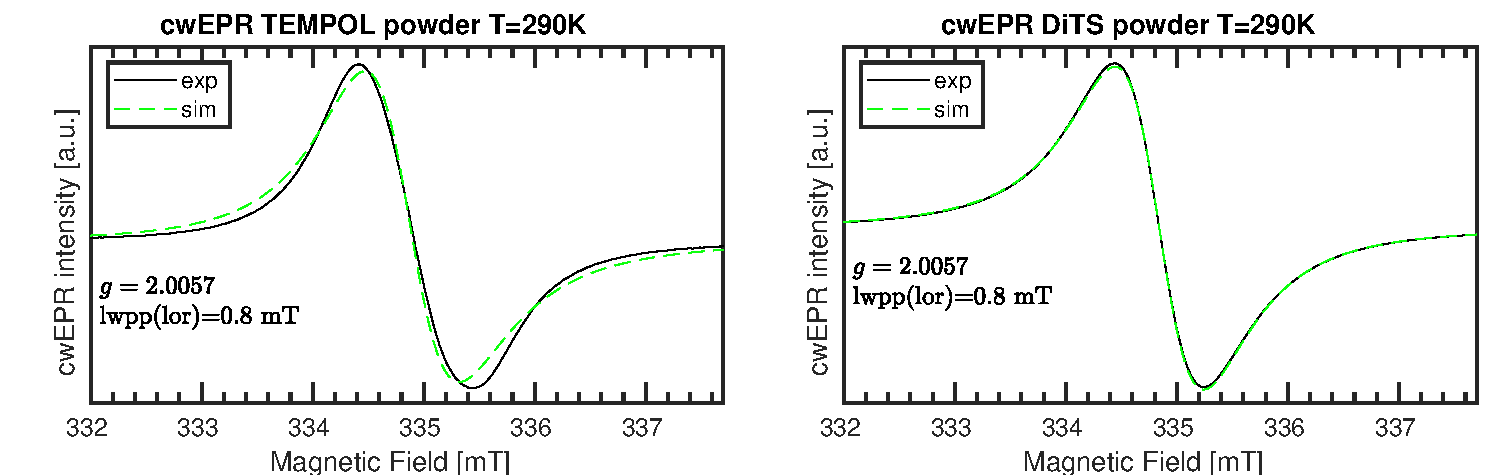
\includegraphics[width=1\textwidth]{./operando_epr/figures/TEMPOL/cwEPR_TEMPOL_vs_DiTS_RT_POWDER.pdf}
	\caption{Room temperature cwEPR spectra of pure TEMPO-containing powders. Left: TEMPO, Right: Di-Tempo-Salen.}
	\label{fig:cwEPR_monoTEMPO_diTEMPO_POWDER}
\end{figure}

\begin{figure}[h]
\center
	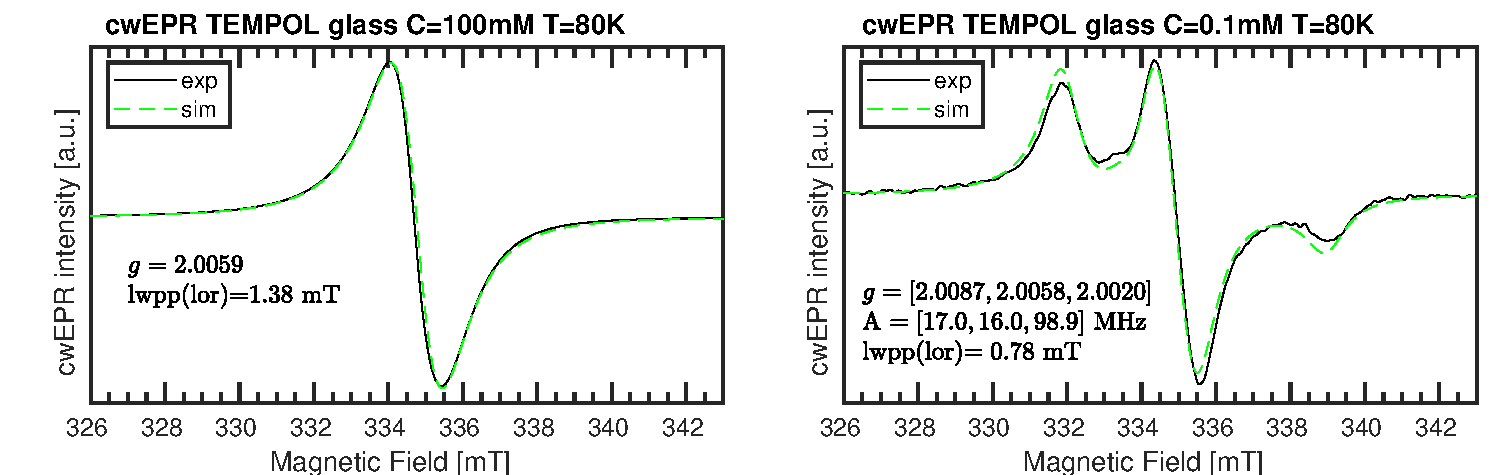
\includegraphics[width=1\textwidth]{./operando_epr/figures/TEMPOL/cwEPR_TEMPOL_100mM_vs_p1mM_80K.pdf}
	\caption{Cryogenic cwEPR spectra of TEMPOL at high and low concentration in a Dichloroethane/Acetonitrile glass. Left: 100~mM, Right: 0.1~mM.}
	\label{fig:cwEPR_TEMPOL_High_Low_Concentrations}
\end{figure}



\par
A biradical molecule like Di-Tempo-Salen (Figure~\ref{},x) has two paramagnetic species that are close to each other and therefore exchange electrons. When the exchange coupling between the radicals $J$ is comparable to the hyperfine coupling $A$ of each radical to its 'host' nucleus, the superhyperfine interaction~\cite{} takes place, in which the radical is interacting to the nucleus of the neighboring radical~\cite{Eaton2018}. Solutions of biradical molecules with magnetic nuclei show more features in cwEPR spectra when the electron-electron exchange coupling $J$ between the two radicals within the molecule becomes comparable to the hyperfine coupling between the radical and its 'host' $^{14}$N nucleus. tumbling of the molecule and the restricted motions of each radical within the molecule cause a complex molecular motion that affects the dipolar and exchange couplings between the radicals and causes "spectra with alternating linewidths"~\cite{Eaton2018,carrington}. A solution of Di-TEMPO-Salen shows a five-line cwEPR spectrum with alternating linewidhts (Figure~\ref{fig:cwEPR_monoTEMPO_diTEMPO}, right) with the three most intense lines corresponding to the three hyperfine sublevels of TEMPO$^{\bullet}$. The five-line structure in the cwEPR spectrum indicates the presence of a di-TEMPO biradical in the solution.




\par
TOLYAN:\\
If the TEMPO groups are far away from each other, their cw-EPR signal consists of three
lines that are due to the hyperfine interaction between the electron spin and the spin of the Nitrogen
nucleus. When the TEMPO groups are brought closer to each other, their electron orbitals start to
overlap, and the exchange interaction (J) between the electrons grows. That splits the signal into
more lines as it was shown by [10] and represented in Fig. 7. In the case of strong exchange
interaction the spectrum consists of five lines with relative ratios 1:2:3:2:1. In the absence of the
exchange interaction the spectrum contains only three hyperfine lines of equal intensities.
In DiTS, a sum of a three-line spectrum and a five-line spectrum was observed. This may
be the evidence that TEMPO-bearing linkers are sufficiently long to allow TEMPO groups to move
freely in space around the organometallic complex. That can yield to different J values depending
on the relative orientation of the linkers, similar to [10]. In theory, there are several possible
positions of TEMPO groups relative to each other that can change the EPR spectrum. Depending
on the angle between the linkers (from $\pi$ to 0), J may vary from its minimal to maximal value,
that should yield a three- and five-line structures respectively. Since the process of movement is
dynamic, we can explain the observed picture as a combination of several positions in space [10].
The five-line structure suggests different preferred conformations of the TEMPO fragments and
dynamic interconversion between these states with different exchange coupling J leads to the
observed spectrum.

\subsection{Spectra of TEMPO$^{\bullet}$/TEMPO$^{+}$ Films}
A film made of a TEMPO-containing polymer can be brought to a certain oxidation state, depending on how many of the TEMPO groups are in the radical (TEMPO$^{\bullet}$) state and how many are in the oxidized (TEMPO$^{+}$) state. The densely packed TEMPO$^{\bullet}$ fragments in the film cannot be considered as isolated molecules anymore, and the interactions between the radicals become significant. Microcrystals of TEMPOL are densely packed TEMPO$^{\bullet}$ with a concentration of $???$~mM. The cwEPR spectrum of TEMPOL in Figure~\ref{fig:cwEPR_TEMPOL_SOLID} is one broad line centered at $g=2.0055$.

\begin{figure}[h]
\center
	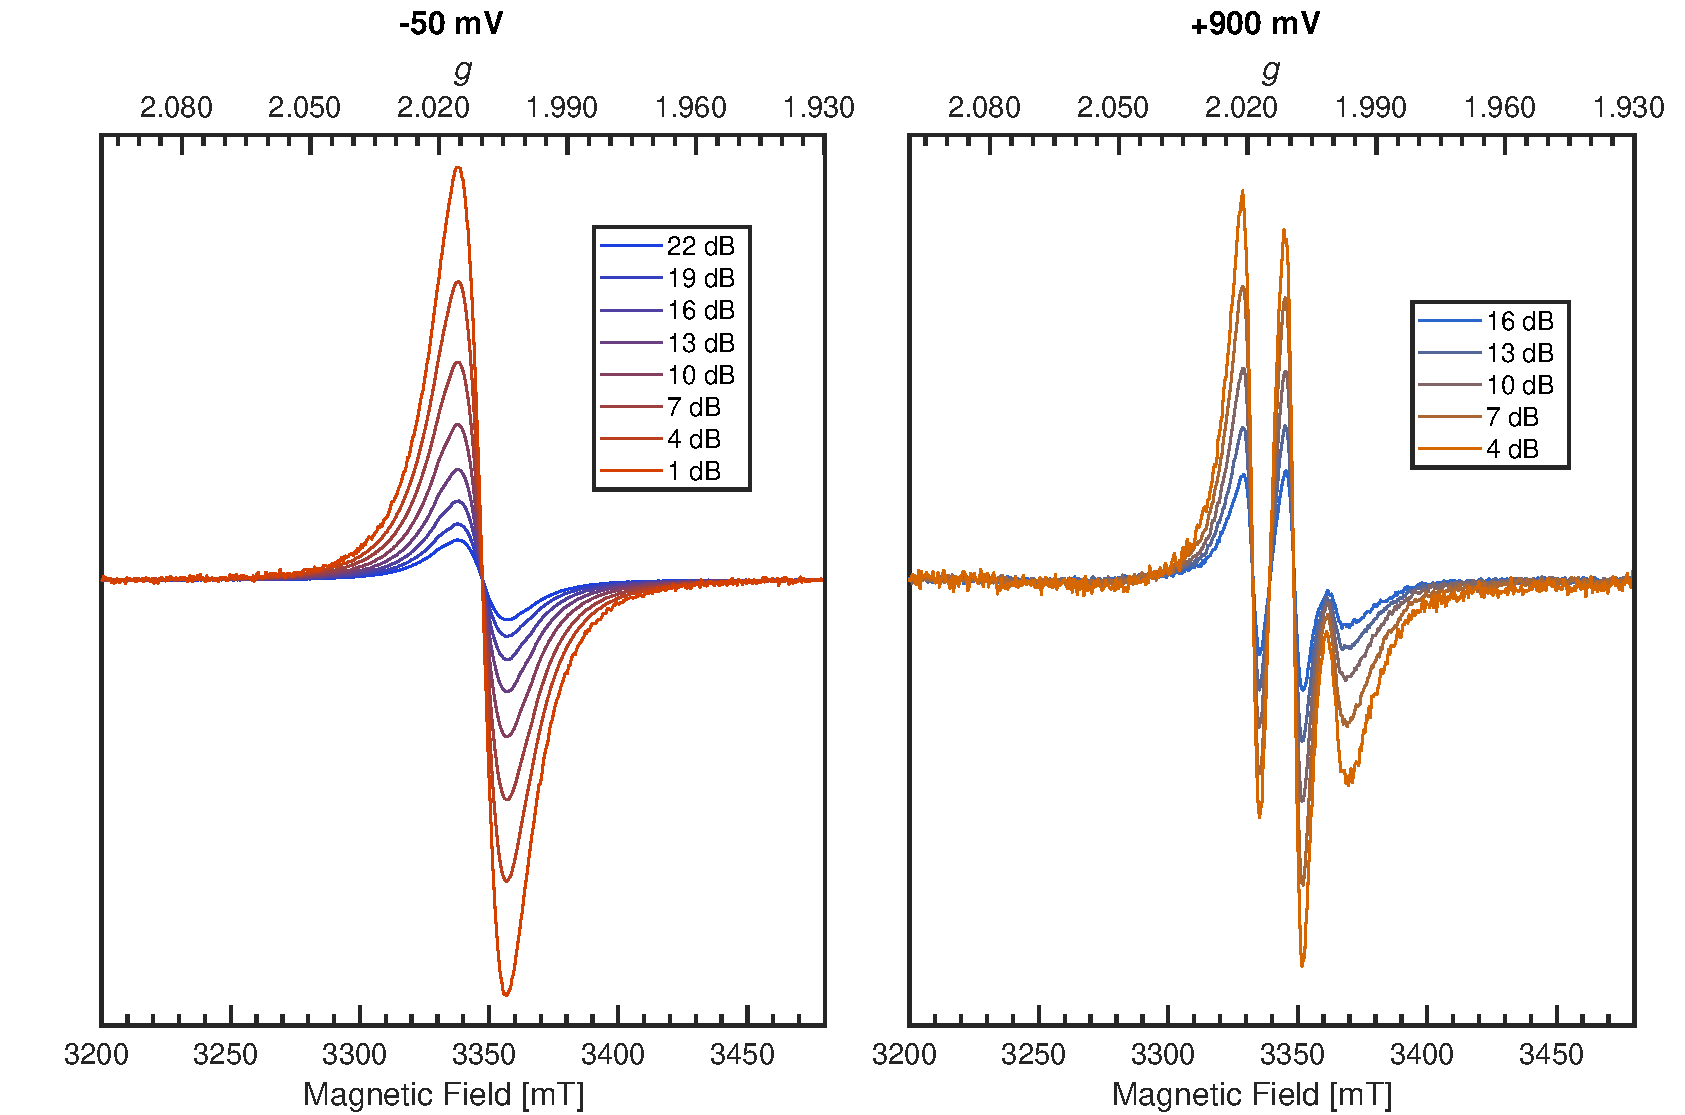
\includegraphics[width=1\textwidth]{./operando_epr/figures/CRYO/S220104_CW.pdf}
	\caption{Cryogenic (80~K) cwEPR spectra of a pDiTBuS film grown with 200 deposition cycles. Left: discharged film, -50~mV vs. Ag/AgNO$_3$ RE. Right: Fully charged film, 900~mV vs. Ag/AgNO$_3$ RE.}
	\label{fig:cwEPR_CRYO_DiTBuS_DCG_vs_CHG}
\end{figure}

\begin{figure}[h]
\center
	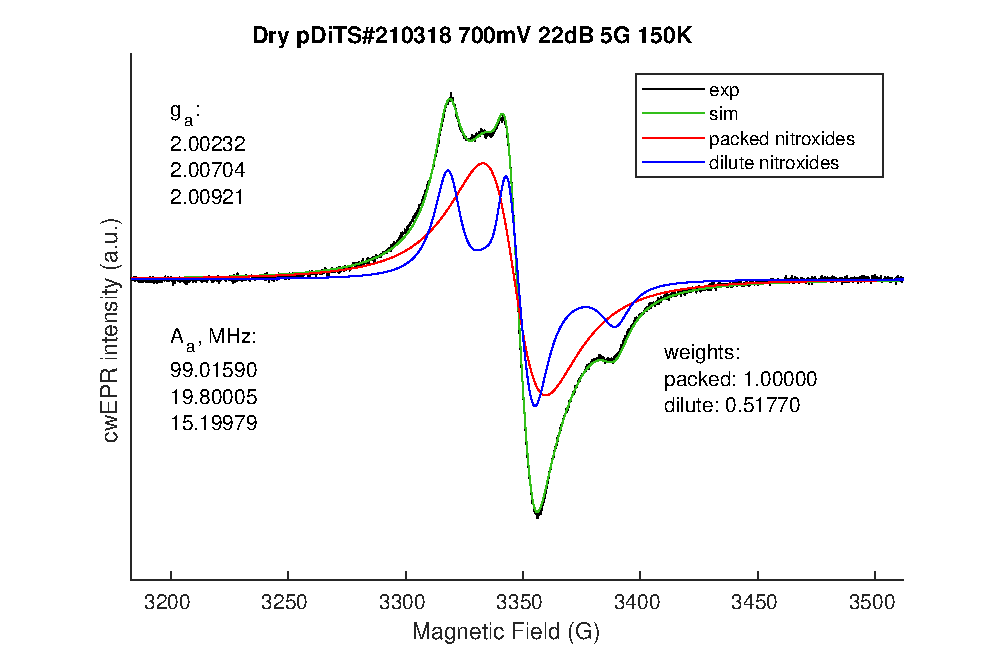
\includegraphics[width=1\textwidth]{./operando_epr/figures/CRYO/cw_sim_pDiTS_210318_700mV_2comp.pdf}
	\caption{A pDiTS film in the intermediate state of charge (700~mV vs. Ag/AgNO$_3$) showing a composition of two spectral signatures. The single-line signal from the densely packed nitroxide radicals coexists with the signal of the isolated nitroxide radicals. Two-component simulation.}
	\label{fig:cwEPR_CRYO_DiTS_2_COMP_SIM}
\end{figure}



\begin{figure}[h]
\center
	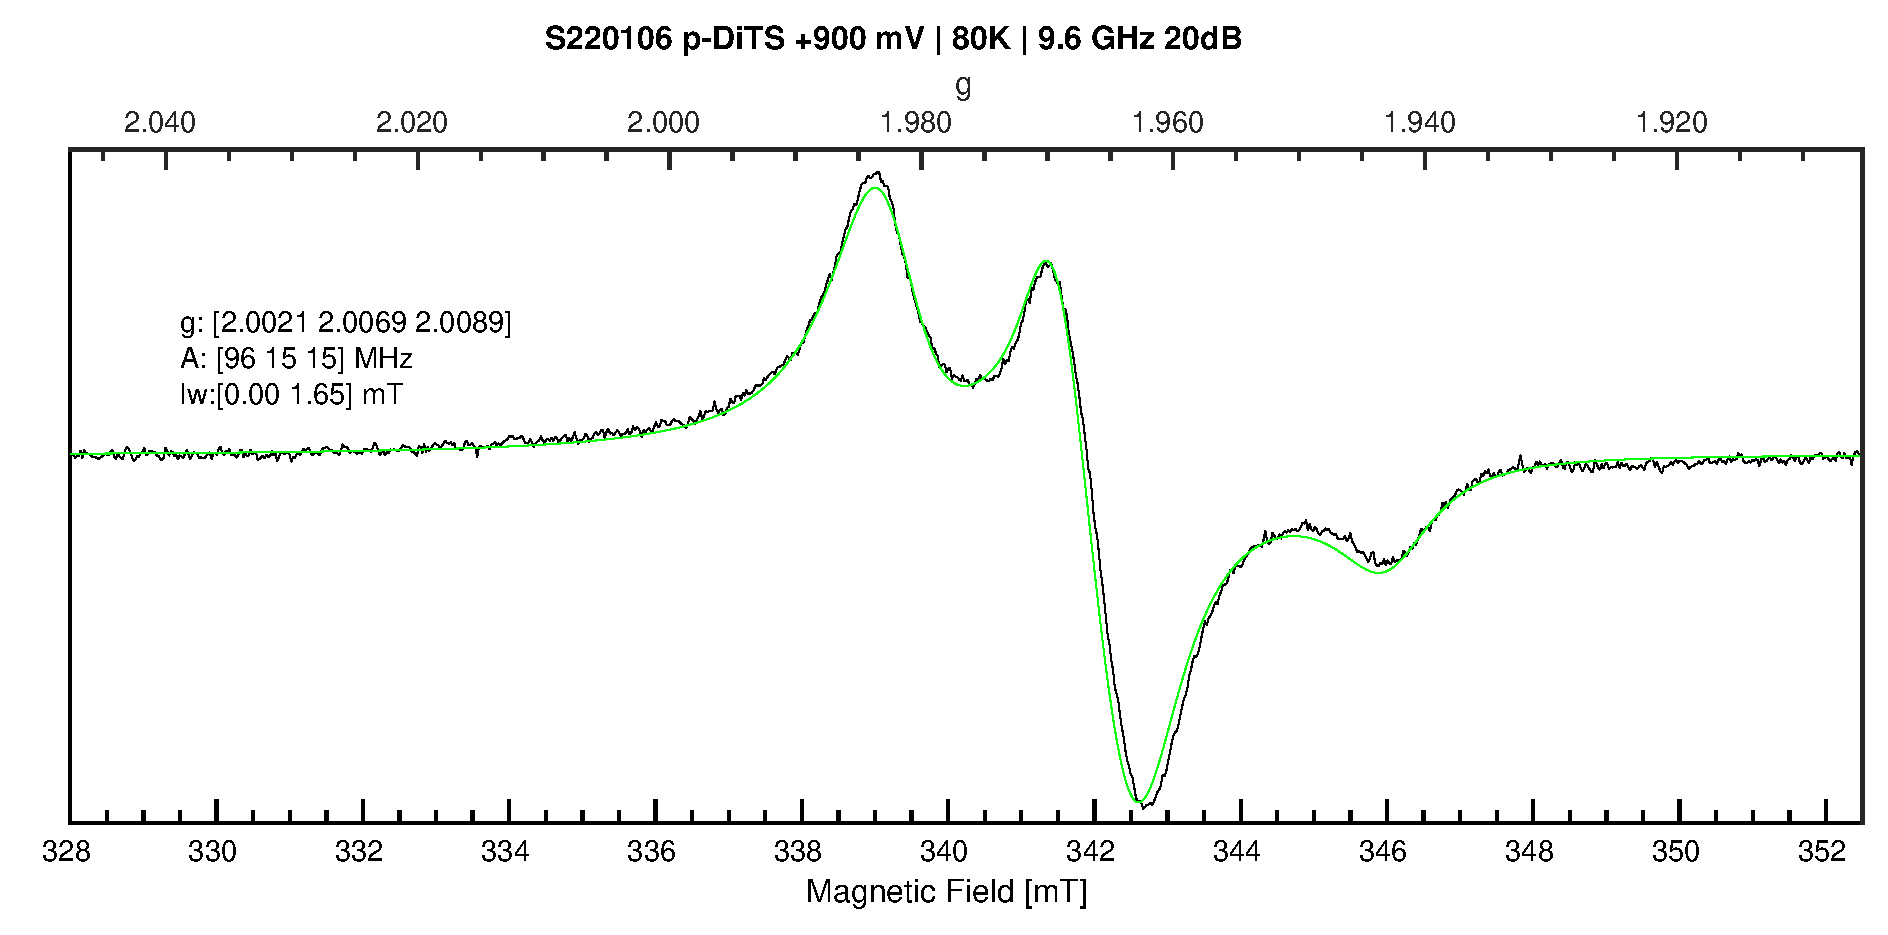
\includegraphics[width=1\textwidth]{./operando_epr/figures/CRYO/S220106_p-DiTS_OX_80K_CW_SIM.pdf}
	\caption{Simulation of the cryogenic (80~K) cwEPR spectrum of an oxidized pDiTBuS film grown with 200 deposition cycles showing a signature of the isolated nitroxide radical with $g=?$ and $A=?$.}
	\label{fig:cwEPR_CRYO_DiTBuS_CHG_SIM}
\end{figure}



\begin{figure}[h]
\center
	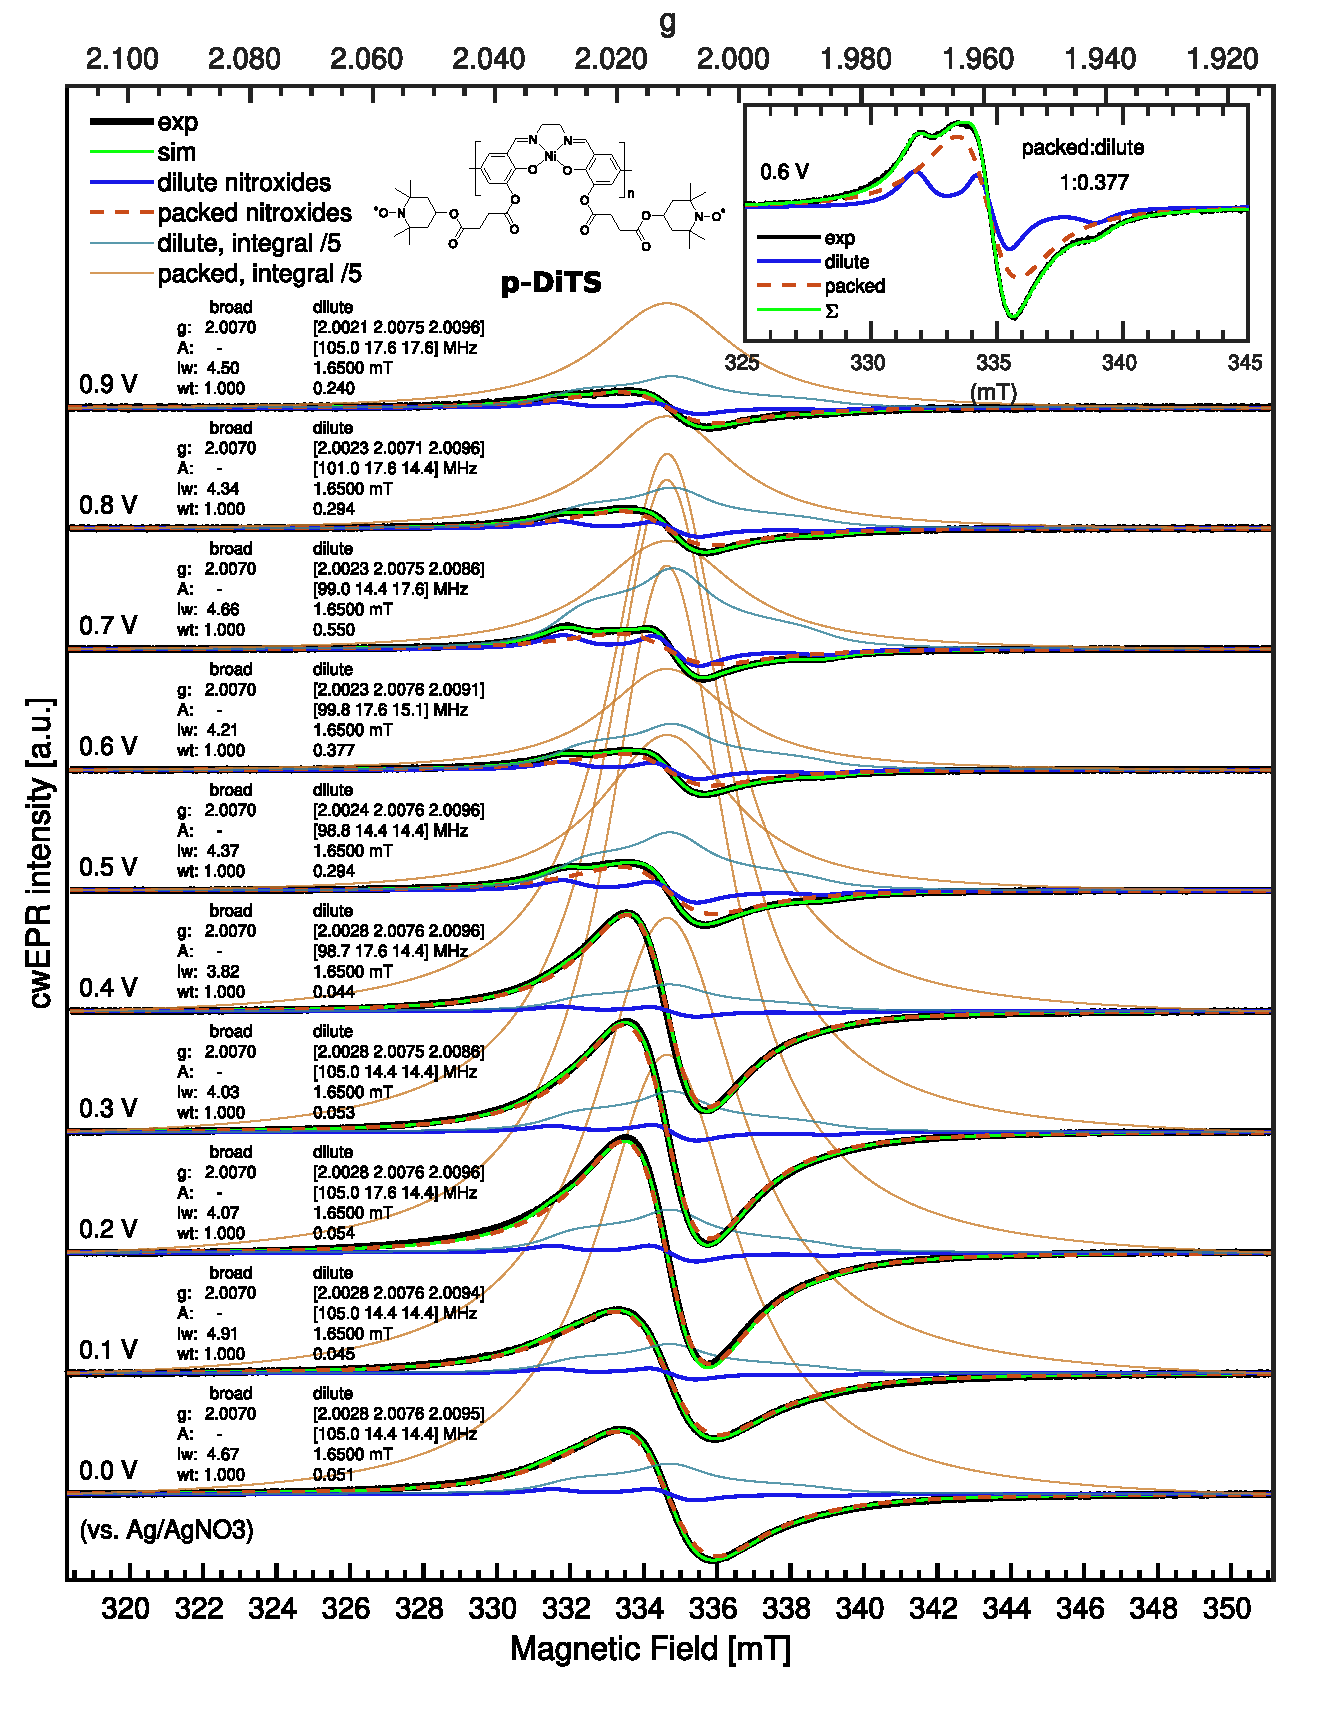
\includegraphics[width=1\textwidth]{./operando_epr/figures/CRYO/Figure_S7_new.pdf}
	\caption{copy from SI.}
	\label{fig:cwEPR_CRYO_DiTS_CHG_SIM}
\end{figure}



\subsection{Spectra of NiSalen Films}
\begin{figure}[h]
\center
	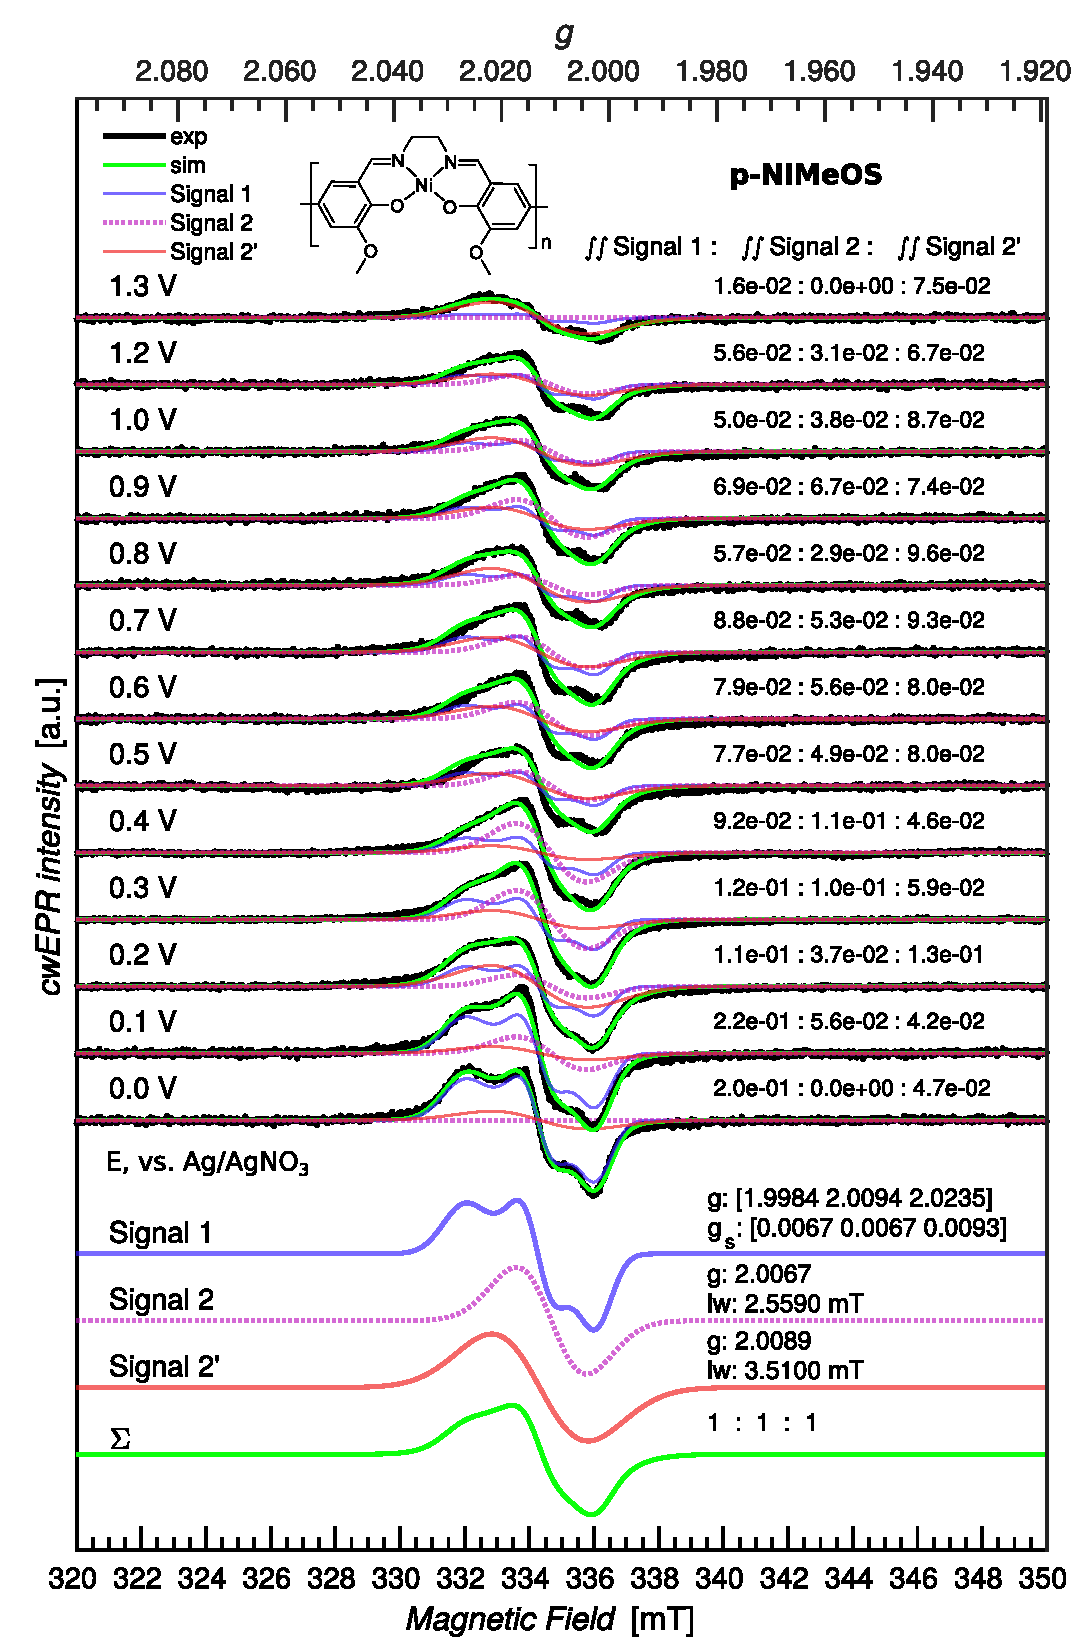
\includegraphics[width=1\textwidth]{./operando_epr/figures/CRYO/Figure_S8.pdf}
	\caption{Potential-dependent cwEPR spectra of a NiMeOSalen film measured at 150~K. Simulation of the spectra with three components reported by the Timonov group.}
	\label{fig:cwEPR_CRYO_NiSalen_REDOX_SIM}
\end{figure}



\section{cwEPR Spectroscopy of a Charging Electrochemical Cell}
There is a number of difficulties when it comes to an EPR experiment on a working electrochemical cell. The cell must contain mobile ions between its electrodes - cations and anions. The ions are normally produced as products of dissociating salts. To overcome the ionic bond in a salt and to break it into the ions, a solvent with large dipole moment is needed. Solvents with large dipole moments, as acetonitrile (CH\textsubscript{3}CN, $\epsilon\approx 37.5$) or water ($\epsilon\approx78.4$), have large dielectric constants which results in a non-resonant absorption of microwaves. A cell containing liquid electrolyte absorbs microwaves and lowers the sensitivity of the EPR experiment. Furthermore, due to a finite dimension of cell, not only the magnetic component of the microwave is interacting with the electrolyte, but also the electric one - this results in heating of the electrolyte in a similar fashion as in a microwave oven. The heating of the electrolyte leads to a faster degradation of the cell and does not allow for long systematic measurements.\\
Another general issue with the operando EPR and EDMR experiments is that the device under testing (DUT) has to have metal electrodes that deliver current to it. Metals, placed in a microwave cavity, change the distribution of the electromagnetic field in it - that weakens the magnetic component at the device and at the same time strengthens the electric component. It is the magnetic dipole transition that is causing the magnetic resonance, so the weakening of the magnetic component by introducing the metal electrodes further decreases the magnetic resonance response. The increased electric component causes heating to temperatures that can be critical for the DUT operation.

\subsection{Fabrication of EPR-compatible Electrochemical Cells}

\section{Versatile electrode setup for ex-situ and in-situ spectroelectrochemical EPR}\label{electrode_setup}
%
There is increasing interest in both ex-situ and in-situ spectroelectrochemical (SEC) EPR measurements in research fields ranging from biology to materials science, from redox active systems such as proteins~\cite{abdiaziz2019_chemcomm} and hydrogenase to catalysis,\cite{kutin2019_catalysis, neukermans2020_chemelectrochem, bonke2021_natrev, priebe2013_angewandte, rabeah2015_angewandte} redox-flow batteries~\cite{zhao2021_jacs} and of course ORBs.\cite{huang2016_jpowersources, kanzaki2018_acsappmat} One significant drawback with SEC EPR is the fact that microwave resonators suffer from substantial microwave damping as a result of introducing metal electrodes, polar solvents and ionic salts (i.e., the electrolyte) needed for successful electrochemistry.\cite{wadhawan2007_encofelectrochem} Microwave damping can be significantly reduced by our novel on-substrate electrode design (see Fig.~\ref{fig:flat_tube}) as this limits the amount of metal that is introduced into the resonator, while still allowing us to have electrode surface areas large enough to deposit sufficient material of interest to observe EPR signals.

\begin{figure*}[ht!]
 \centering
 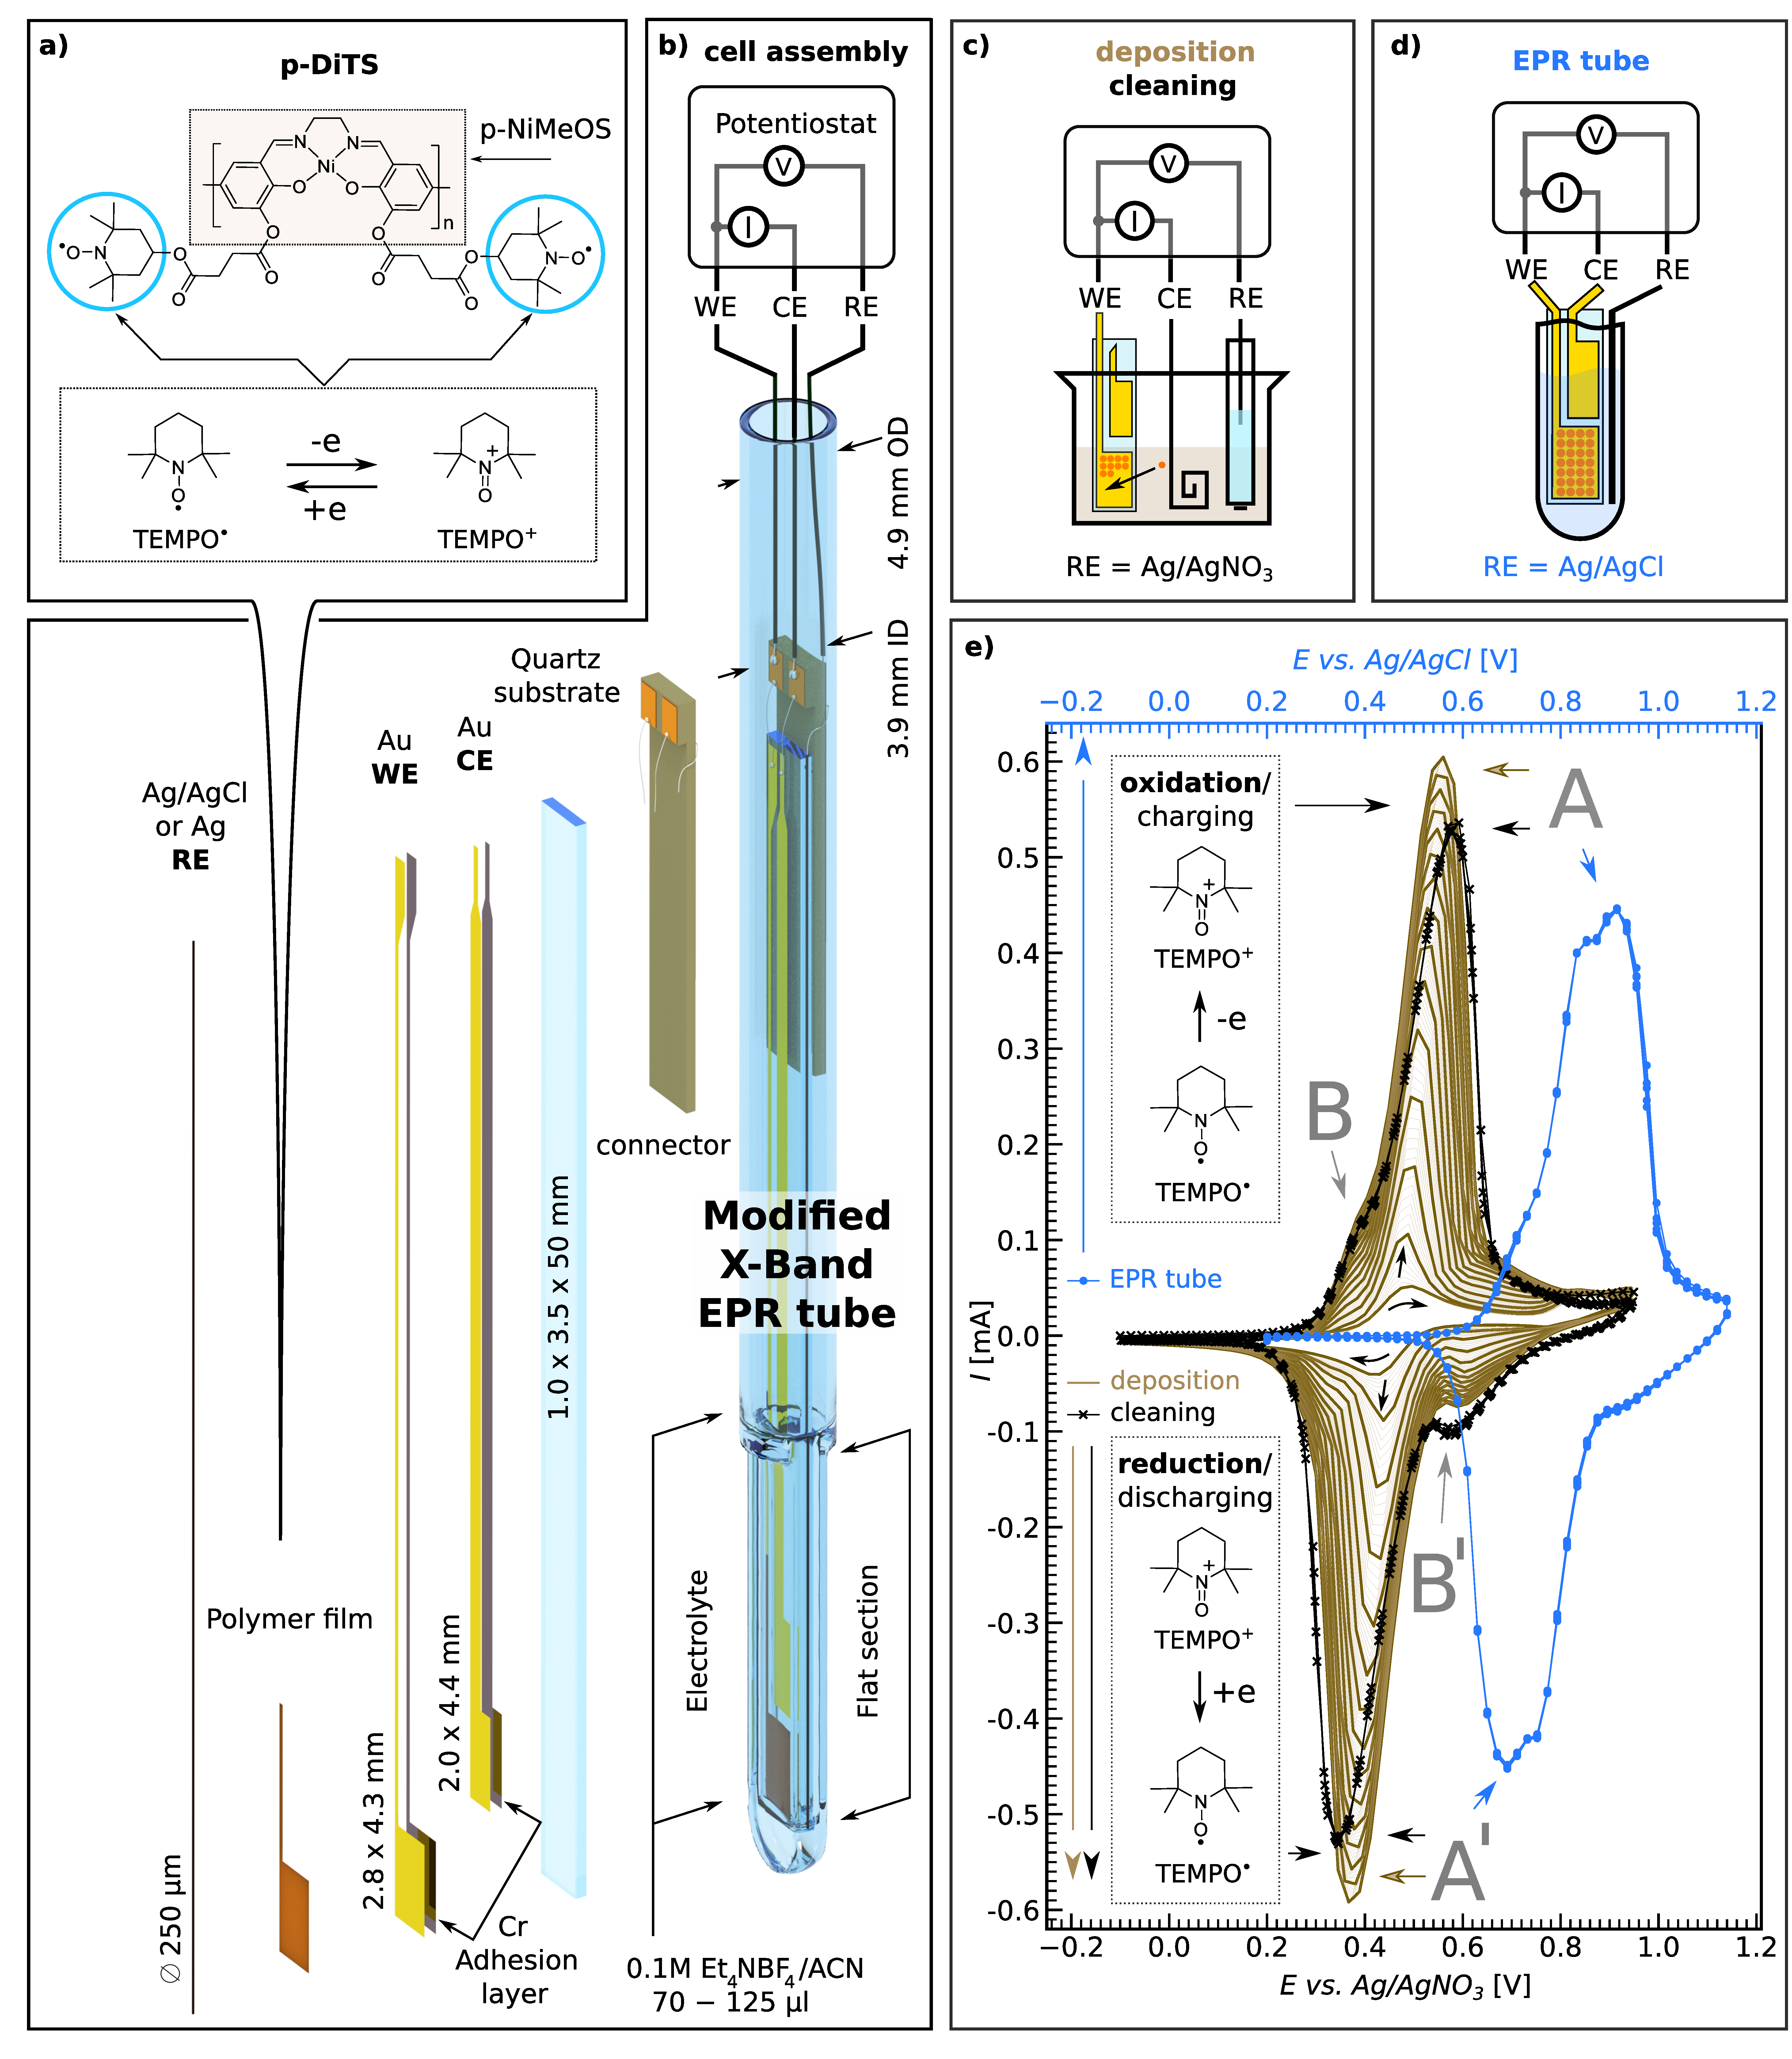
\includegraphics[width=0.99\textwidth]{./operando_epr/figures/Flat_tube_setup.pdf}
 \caption{Schematic diagram of the electrode design and assembly of the electrochemical cell based on a modified X-band EPR quartz tube. a): Molecular structure of p-DiTS, with the redox reaction of its charge-bearing TEMPO groups; highlighted is the backbone, p-NiMeOSalen. b): Photograph of the modified tube with a flattened bottom section, with the on-substrate electrochemical setup assembled inside, and the process of forming the modified tube. c): Electrochemical setup for deposition and cleaning of polymer films. d): Tube-based electrochemical setup. e): Cyclic voltammograms of a growing p-DiTS film during 100 electropolymerization cycles (solid-brown), during the cleaning process (crossed-black) and in the tube-based setup (dotted-blue). Peaks A/A', B/B' correspond to the oxidation and reduction of the TEMPO fragments and of the p-NiSalen backbone, respectively. All CV were recorded at 50~mV\,s\textsuperscript{-1}.}
 \label{fig:flat_tube}
\end{figure*}

\par
The on-substrate electrodes are produced as follows. Cleaned quartz substrates are placed inside a holder and covered with shadow masks. The assembly is transferred into a vacuum chamber equipped with a thermal evaporator (MBraun ProVap 5G PVD System). At a pressure of $7\times10^{-7}$~mbar, 10~nm of Chromium (Cr) adhesion layer is evaporated, followed by 180~nm of Gold (Au). In this way the on-substrate working and counter electrodes are formed (WE and CE respectively). The reference electrode (RE) is not evaporated on substrate for electrochemical stability reasons. Instead, a \SI{250}{\micro\meter} Ag wire is used, either as is or, for additional stability, coated galvanically with a AgCl layer.\cite{Safari2011} See Section \ref{Experimental_Section} in the ESI$\dag$ for details of the sample preparation.
\par
The above procedure provides a WE active area of 12.0~mm$^2$ which allows one to deposit an electrochemically active film that is large enough to yield a clear EPR signal. The flat electrode design provides the possibility to increase the WE area for samples with particularly small EPR signals while still maintaining certain film thicknesses. This also allows for studying EPR properties as a function of film thickness. In cases where the electrochemical process is thought to deposit material on both the WE and CE, the distance between the on-substrate electrodes can be adjusted such that only one of the electrodes is positioned in the active volume of the microwave resonator, allowing for selective EPR probing of either of the electrodes.
\par
The on-substrate electrodes reduce microwave damping. However, a substantial amount of microwave damping occurs due to the electrolyte, made of polar solvent and ionic salts. Therefore, we further optimize our setup by modifying conventional 5~mm outer diameter (OD) quartz EPR tubes by flattening the bottom 1.3$-$1.6~cm (cf.\ Fig.~\ref{fig:flat_tube}b and Section \ref{fig:S1_modified_tube} in the ESI$\dag$), thereby reducing the active electrolyte volume needed to submerge both the WE and CE on the substrate as well as the RE wire, from $\sim$120~$\mu^{\bullet}$L to $\sim$60$-$70~$\mu^{\bullet}$L.
\par
The flattened tube and the thin-film electrode setup have an additional benefit in that the sample is moved away from the maximum of the electric field distribution in the Bruker ER~4122-SHQE resonator (TE\textsubscript{011} mode cavity for cwEPR), thereby further increasing the resonator quality factor (Q-factor, given by $Q = \frac{\nu_{res}}{\Delta \nu}$, $\nu_{res} =$ resonance frequency, $\Delta \nu =$ FWHM of the resonance dip) and hence sensitivity. Further improvements can be made using the flat electrode setup in a TM\textsubscript{110} mode cwEPR cylindrical cavity such as a Bruker ER~4103-TM (developed for studying samples exhibiting high dielectric constants), where the flattened cell can be aligned to further reduce coupling to the microwave electric field. The modified tube is compatible with commercial Bruker ER~4118X-MD5 resonators, most commonly used for advanced pulse EPR measurements at X-band frequencies ($\nu = 9-10$~GHz).


\subsection{Fabrication of the modified tube}
%
The volume of the cell used in this study had to be minimized, as the high dielectric constant of the electrolyte does not allow for the critical coupling of the resonator. The volume of the electrolyte was minimized by flattening the tip of the quartz (melting point $T_m=1660-1710\,^{\circ}$C) tube accommodating the cell. For that, a tungsten (W, $T_m=3420\,^{\circ}$C) rod of a 3.70$\times$1.35$\,$mm rectangular cross section, narrowing to the bottom of the tube at a wedge angle of $\alpha \approx 5 ^{\circ}$, was inserted into the tube (Fig.~\ref{fig:S1_modified_tube}). The tube was evacuated and filled with He to a pressure of 100~mbar. The tip of the evacuated tube was molten around the thermally expanded rod with a Hydrogen-Oxygen burner ($T_f = 3080\,^{\circ}$C). The modified tube was then connected to atmosphere and the cooled, contracted rod was removed and later reused for modifying other tubes. The tungsten rod was fabricated from an electrode of a flash lamp of a pulsed Nd:YAG laser.\\

\begin{figure*}[h!]
\centering
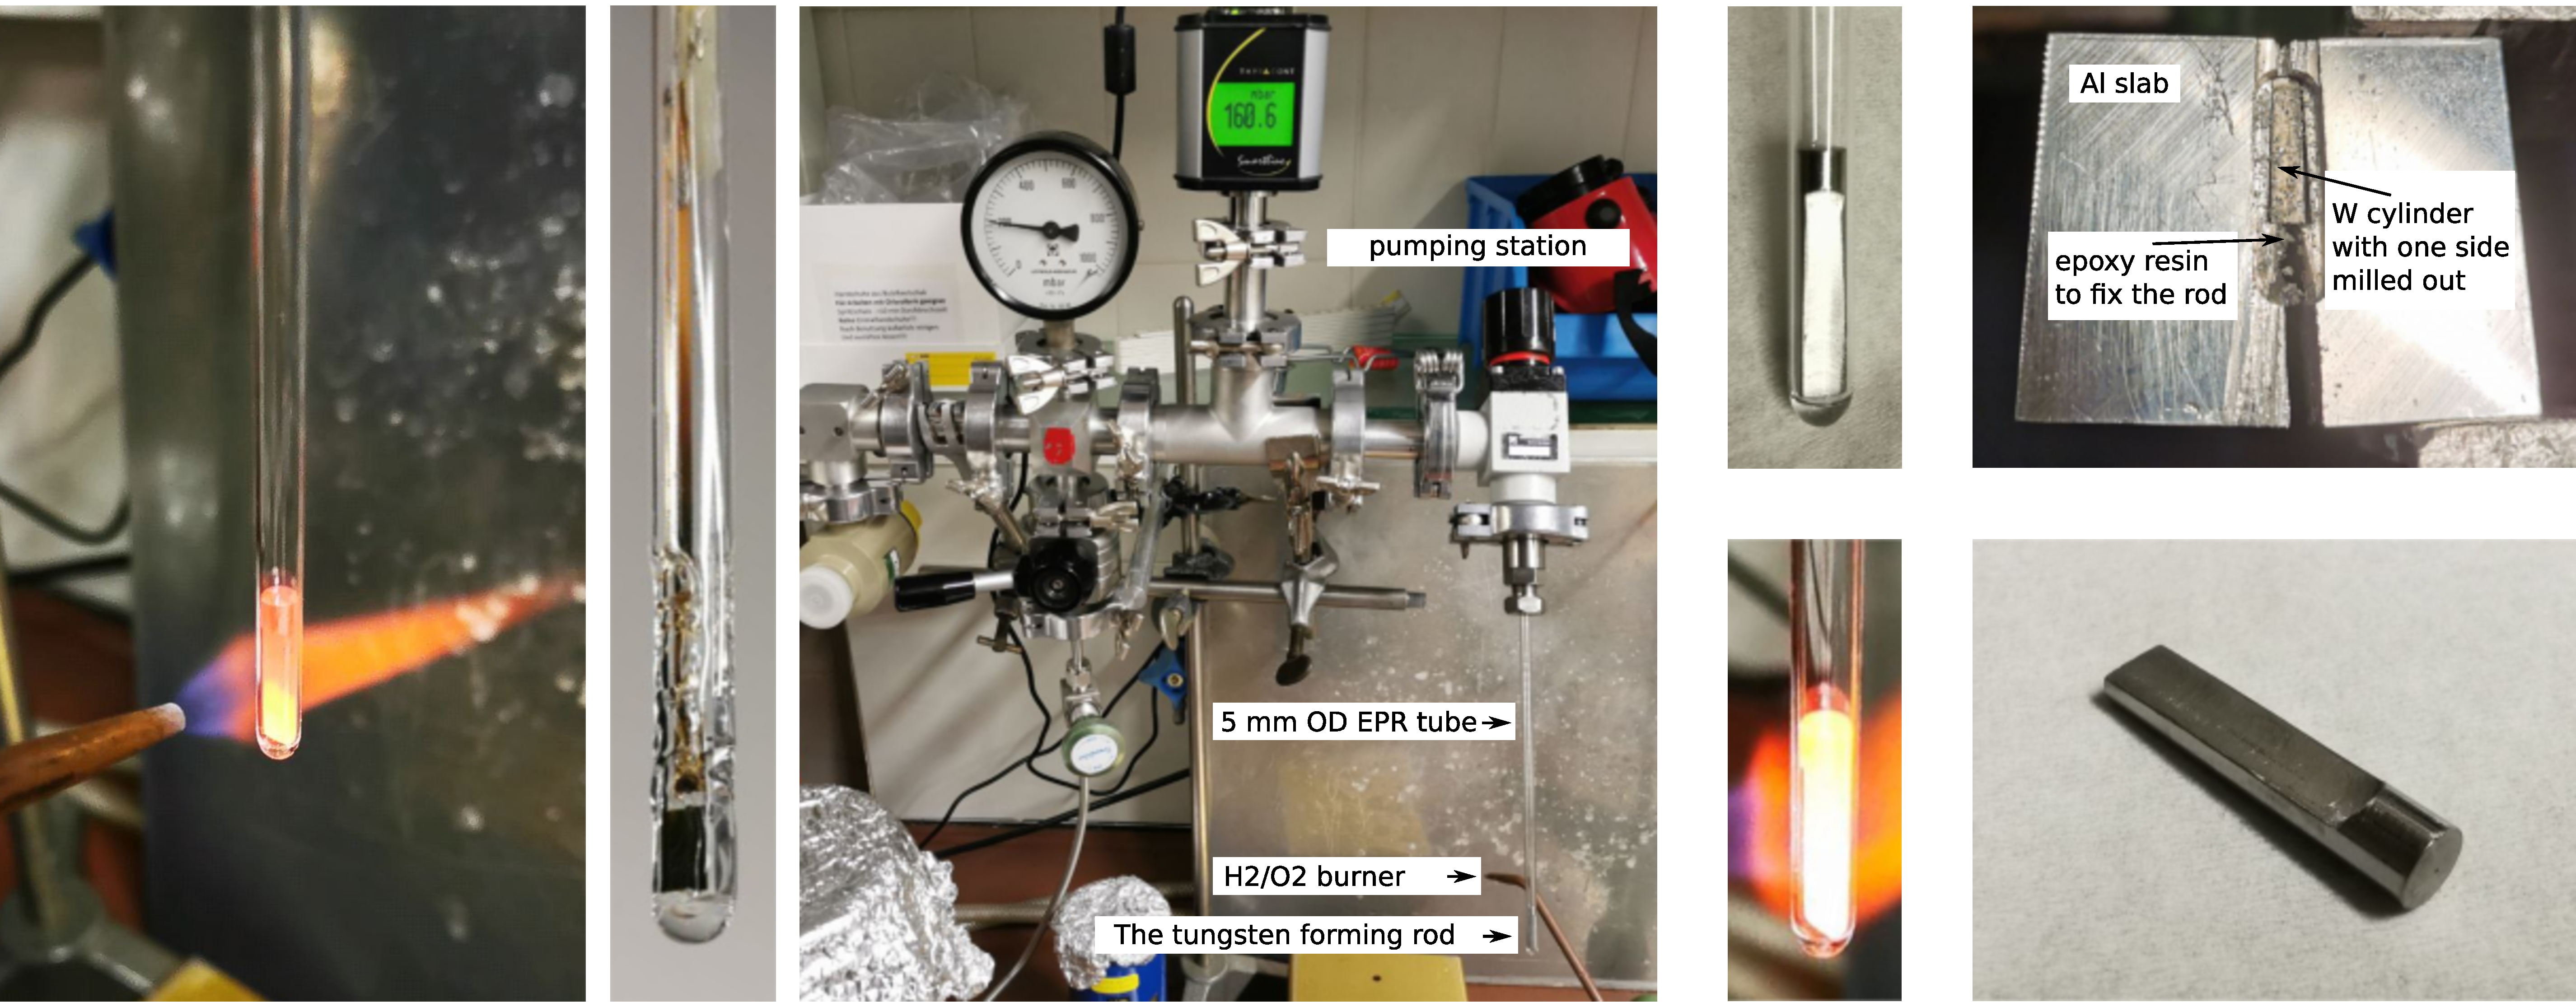
\includegraphics[width=1\textwidth]{./operando_epr/figures/spins_at_work/Figure_S1.pdf}
\caption{Modifying the tip of the standard 5~mm OD quartz EPR sample tube by melting it around a Tungsten (W) forming rod with a H$_2$/O$_2$ burner in an evacuation setup.}
\label{fig:S1_modified_tube}
\end{figure*}

The modification of the tip of the tube provided a decrease in the volume of the electrolyte down to \SI{45}{\micro\liter}, while the cylindrical part of the tube allowed for fitting the substrate connector and the wiring in. That allowed for the room temperature EPR measurements on the electrochemical cell during charging and discharging. Extensive care had to be taken to reproduce the cv curve in the modified tube as the limited volume of the electrolyte was distributed over the large surface area. That caused poor ionic transport in the electrolyte layer.\\


To establish the extent to which the modified tube improves the resonator Q-factor (Q) and therefore sensitivity of the cwEPR experiment, cwEPR spectra and associated Q-factors were recorded for a flat-electrode p-DiTS cell assembled in two different sample tubes. For both cell setups we used enough electrolyte to submerge all three electrodes. This required 100~$\mu^{\bullet}$L for the standard tube and 70~$\mu^{\bullet}$L for the modified tube. The effect of the two tubes on the cwEPR spectrum and on the Q-factor was studied for a range of heights ($H$) measured from the center of the microwave resonator to the middle of the WE.

\begin{figure}[h]

	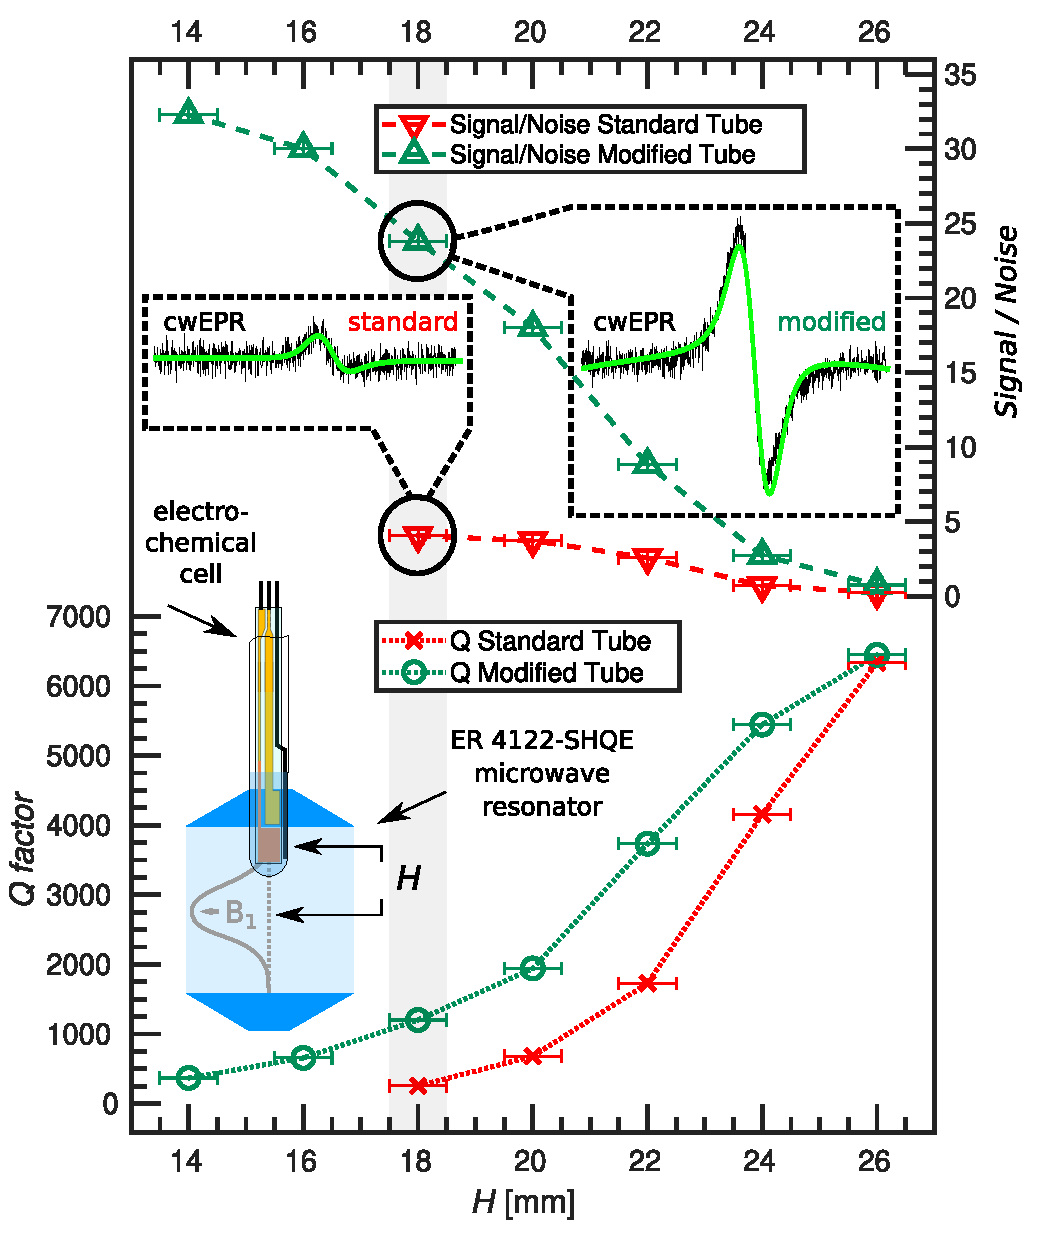
\includegraphics[width=0.5\textwidth]{./operando_epr/figures/Q_factors_mod_tube.pdf}
	\caption
	{Signal-to-noise ratio of the cwEPR spectrum of p-DiTS and the Q-factor of the Bruker ER4122-SHQE microwave resonator measured for an electrochemical cell based on a standard X-band EPR sample tube and for an electrochemical cell based on the modified tube. Data for various heights $H$ from the center of the resonator. Insets: Representative cwEPR spectra at $H=18$~mm, where the signal for the standard tube is the strongest.}
	%{Changes in the microwave resonator Q-factor when loaded with a p-DiTS sample with electrolyte in a standard and modified tube as a function of $H$.}
	\label{fig:Q_factors_mod_tube}
\end{figure}


\subsection{Q-factors and cwEPR spectra for p-DiTS in standard and modified tube}\label{Q-factor_SNR}

We determine Q~$\approx$~7800 for the empty resonator. Inserting the tube-based cells initially at $H=$~24~mm reduces the Q-factor for both cases, but more significantly for the standard tube (Q\textsubscript{standard tube}~$\approx$~4200, Q\textsubscript{modified tube}~$\approx$~5400, see Fig.~\ref{fig:Q_factors_mod_tube}). At $H=$~18~mm the Q-factor drops for both, again more significantly for the standard tube to Q\textsubscript{standard tube}~$\approx$~300 while for the modified tube it is still Q\textsubscript{modified tube}~$\approx$~1200, a factor of 4 difference. This difference between the two tubes shows the benefit of using the modified tube and flat electrode geometries for SEC EPR. When the modified tube is inserted as deep as $H=$~14~mm, the Q\textsubscript{modified tube} is around 400, which still allows for EPR measurements. Coupling the resonator not possible for $H<18$~mm (standard tube) and $H<14$~mm (modified tube).

\par
The decreasing Q-factor is not the only effect of a high-dielectric sample in an EPR resonator. The interaction between the sample and the electric field distribution of the resonator causes a mixture of absorption and dispersion signals, leading to asymmetric lineshapes in the cwEPR spectra. This makes double integration of the derivative cwEPR signal more complex, thereby making a quantitative analysis more difficult. This effect can be seen in the cwEPR spectra of p-DiTS (Fig.~\ref{fig:Q_factors_mod_tube}) measured in the standard 5~mm tube for $H=$~18~mm where the cwEPR signal is asymmetric. The modified tube yields symmetric lineshapes at the same sample heights. Further details are presented in the following subsection.

\par

The electrochemical cells based on the modified tube allow for higher EPR signals as compared to the normal X-band EPR tube. Fig.~\ref{fig:S2_Qfactor} represents two sets of measurements that describe the enhancement of the EPR signal for the modified tube. When the cell is inserted closer to the resonator's center, the Q factor of the resonator lowers and the EPR signal increases, because the intensity of the magnetic component of the microwave field B$_1$ is higher in the center of the resonator. When the cells were inserted closer to the center of the resonator, the Q factor went from $\approx$~6000 down to $\approx$~400, so that the microwave bridge could not be critically coupled to the resonator and no EPR measurements were possible. Depending on the volume of the electrolyte in the cell, it can be inserted more or less deep into the resonator.

The modified tube could be inserted 7 mm deeper into the microwave resonator (see Fig.~\ref{fig:S2_Qfactor}). The EPR signal in the modified tube is increased as compared to the normal tube at the same height.

\begin{figure*}[h!]
\centering
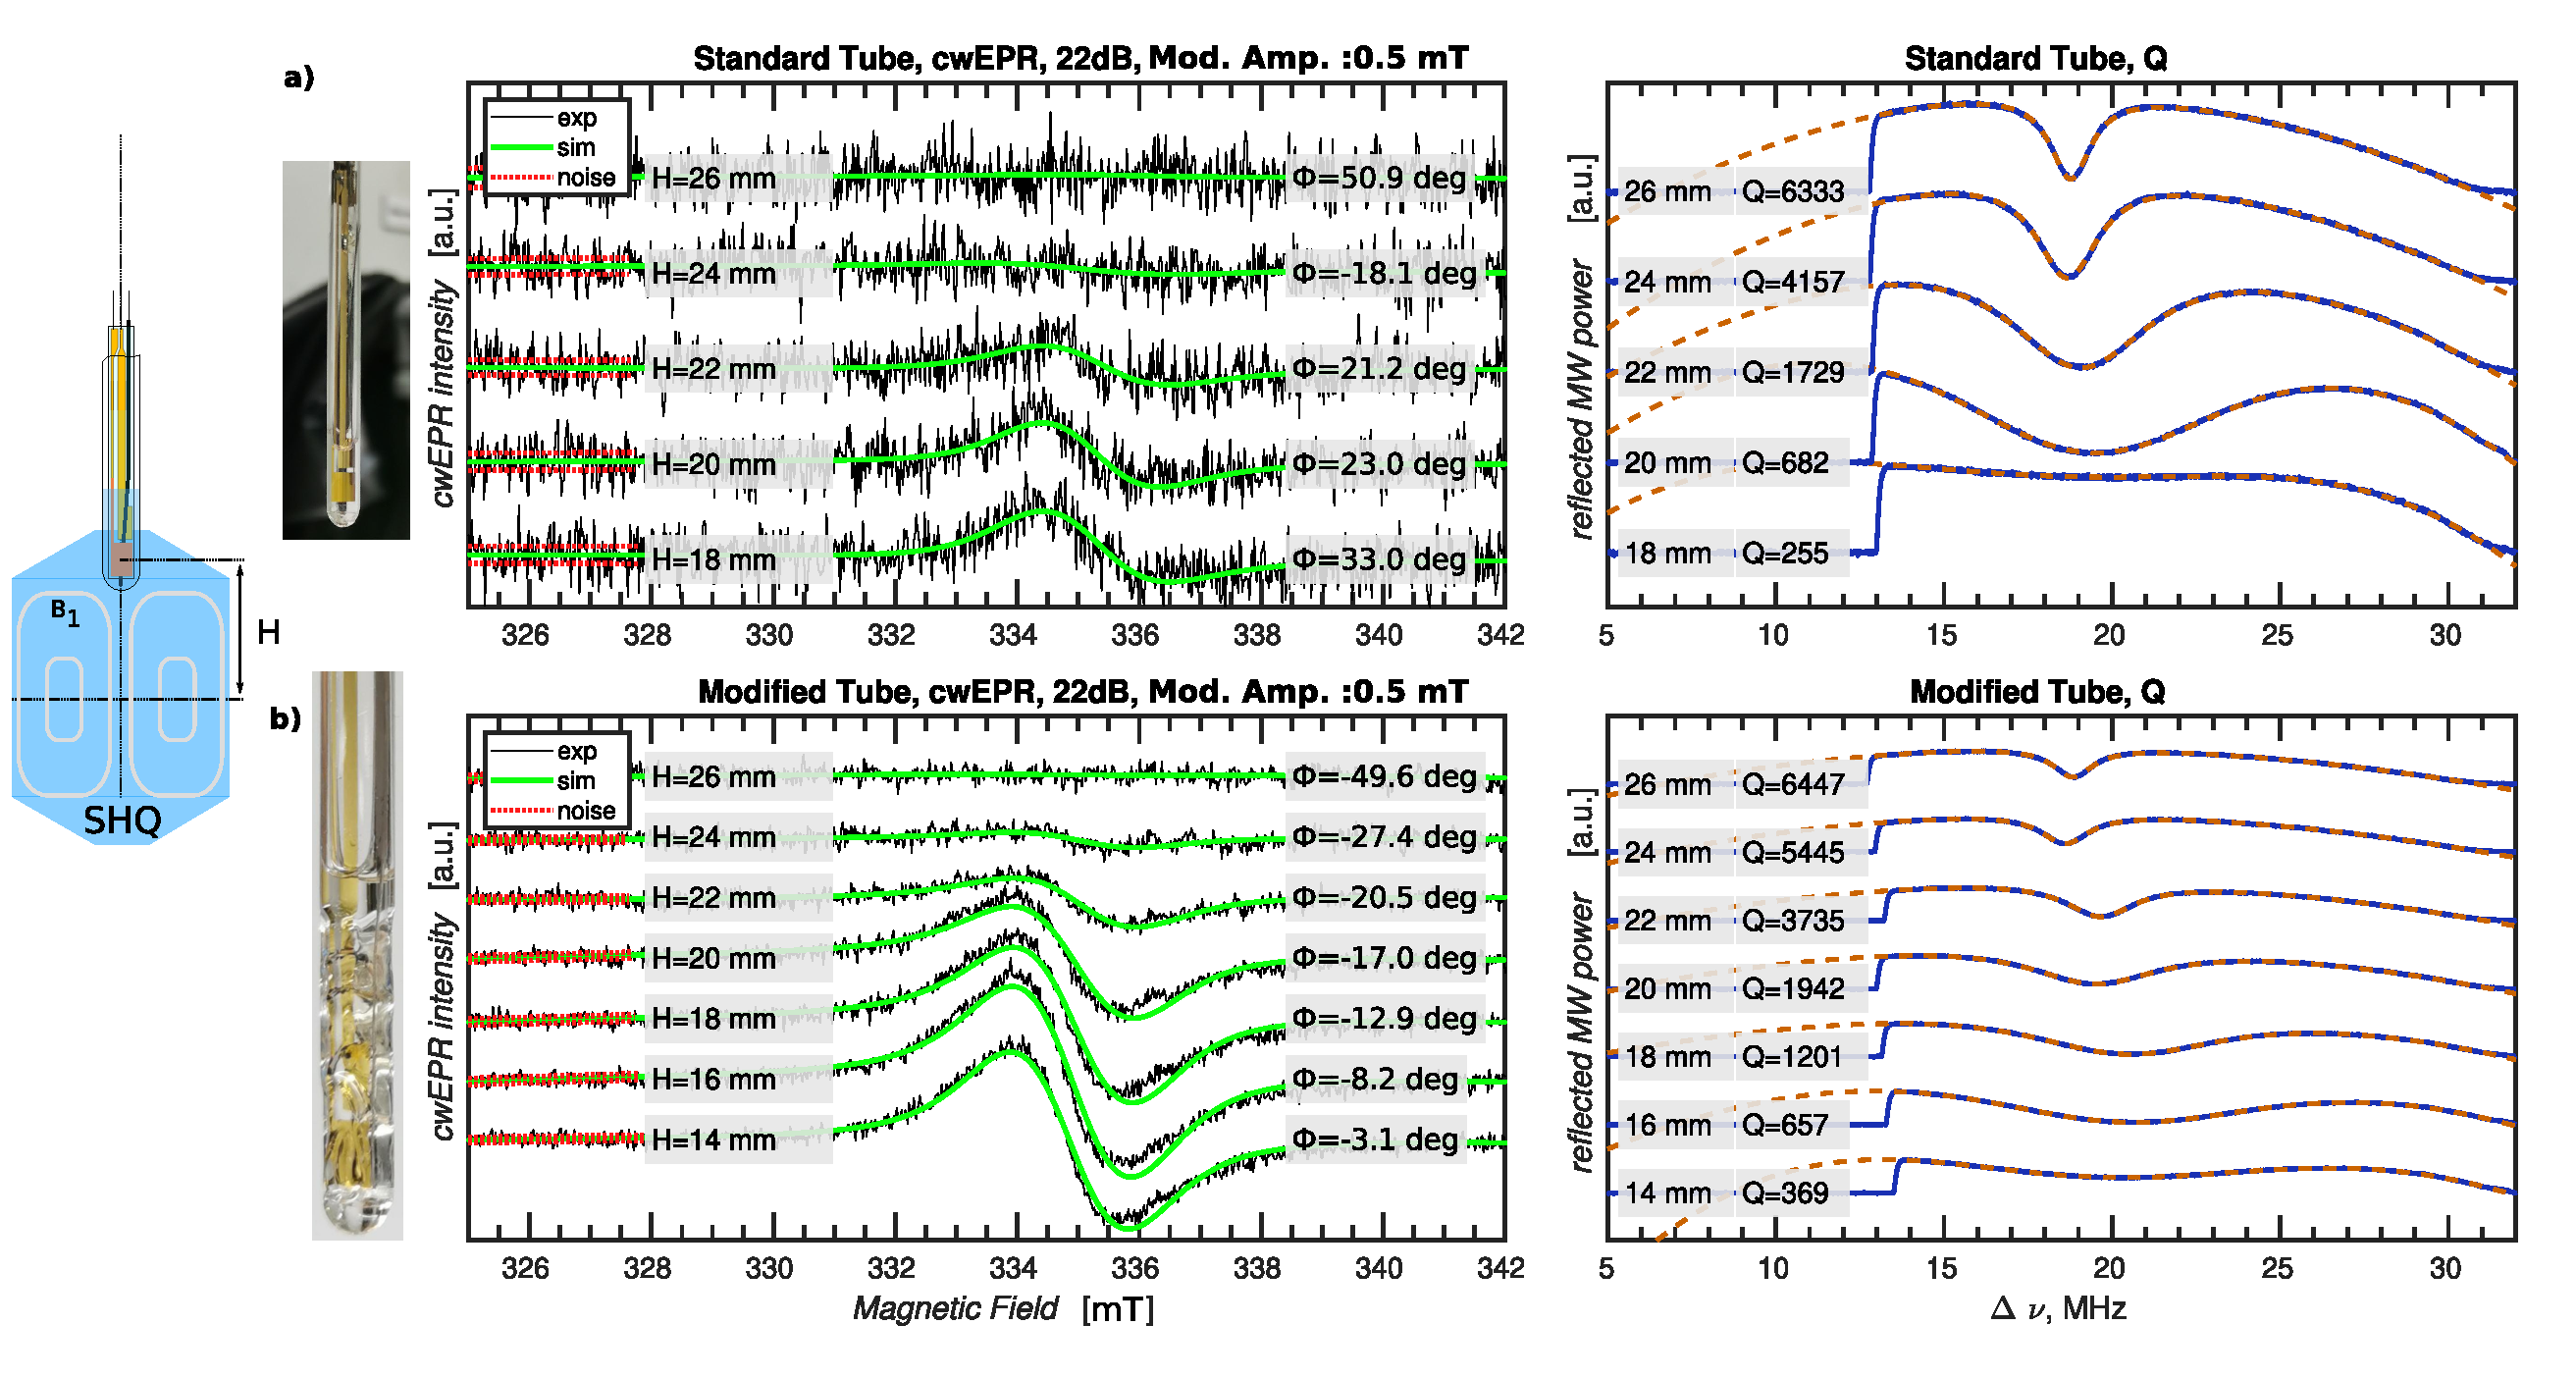
\includegraphics[width=1\textwidth]{./operando_epr/figures/spins_at_work/Figure_S2.pdf}
\caption{cwEPR signal intensity and Q factors for the standard 5~mm OD quartz EPR sample tube and for the modified tube at different heights from the center of the Bruker ER~4122-SHQE resonator. $\nu=$~9.4~GHz. Simulations of the cwEPR spectra with adjusted microwave phase. Noise analysis.}
\label{fig:S2_Qfactor}
\end{figure*}

\par
The modified tube also allows for larger cwEPR signal intensities as it can be inserted closer to the resonator center. The signal-to-noise ratio (S/N) for the modified tube is increased by a factor of $\approx$6 as compared to the standard tube, both inserted at $H=$18~mm. At the maximum sample insertion, the S/N is improved by a factor of $\approx$8 for the modified tube.
\par
Using the modified tube we see three major benefits. Firstly, it results in much higher Q-factors and therefore sensitivity when comparing Q-factors for the same sample height. Secondly, the modified tube allows for insertion of the tube closer to the resonator center, allowing for a larger S/N and therefore requiring less averaging time for each cwEPR measurement. This is especially useful for samples where holding the potential for long periods causes unwanted effects or degradation. Thirdly, cwEPR measurements with the modified tube give symmetric cwEPR lineshapes (using the conventional procedure for critically coupling the microwave cavity, the standard tube gives an asymmetric lineshape) which allows for more straightforward quantitative analysis (spin counting), especially useful for in-situ cwEPR with varying redox potentials.








\subsection{cwEPR Spectra During a Charge-Discharge Cycle}
There are four characteristic cwEPR signatures of an electrochemical cell containing di-TEMPO-Salen polymer cathode. The well known signature of a freely tumbling TEMPO$^{\bullet}$ exhibits three narrow lines corresponding to the three nuclear sublevels of nitrogen: $m_I=-1,0,+1$.
\begin{figure}[h]
\center
	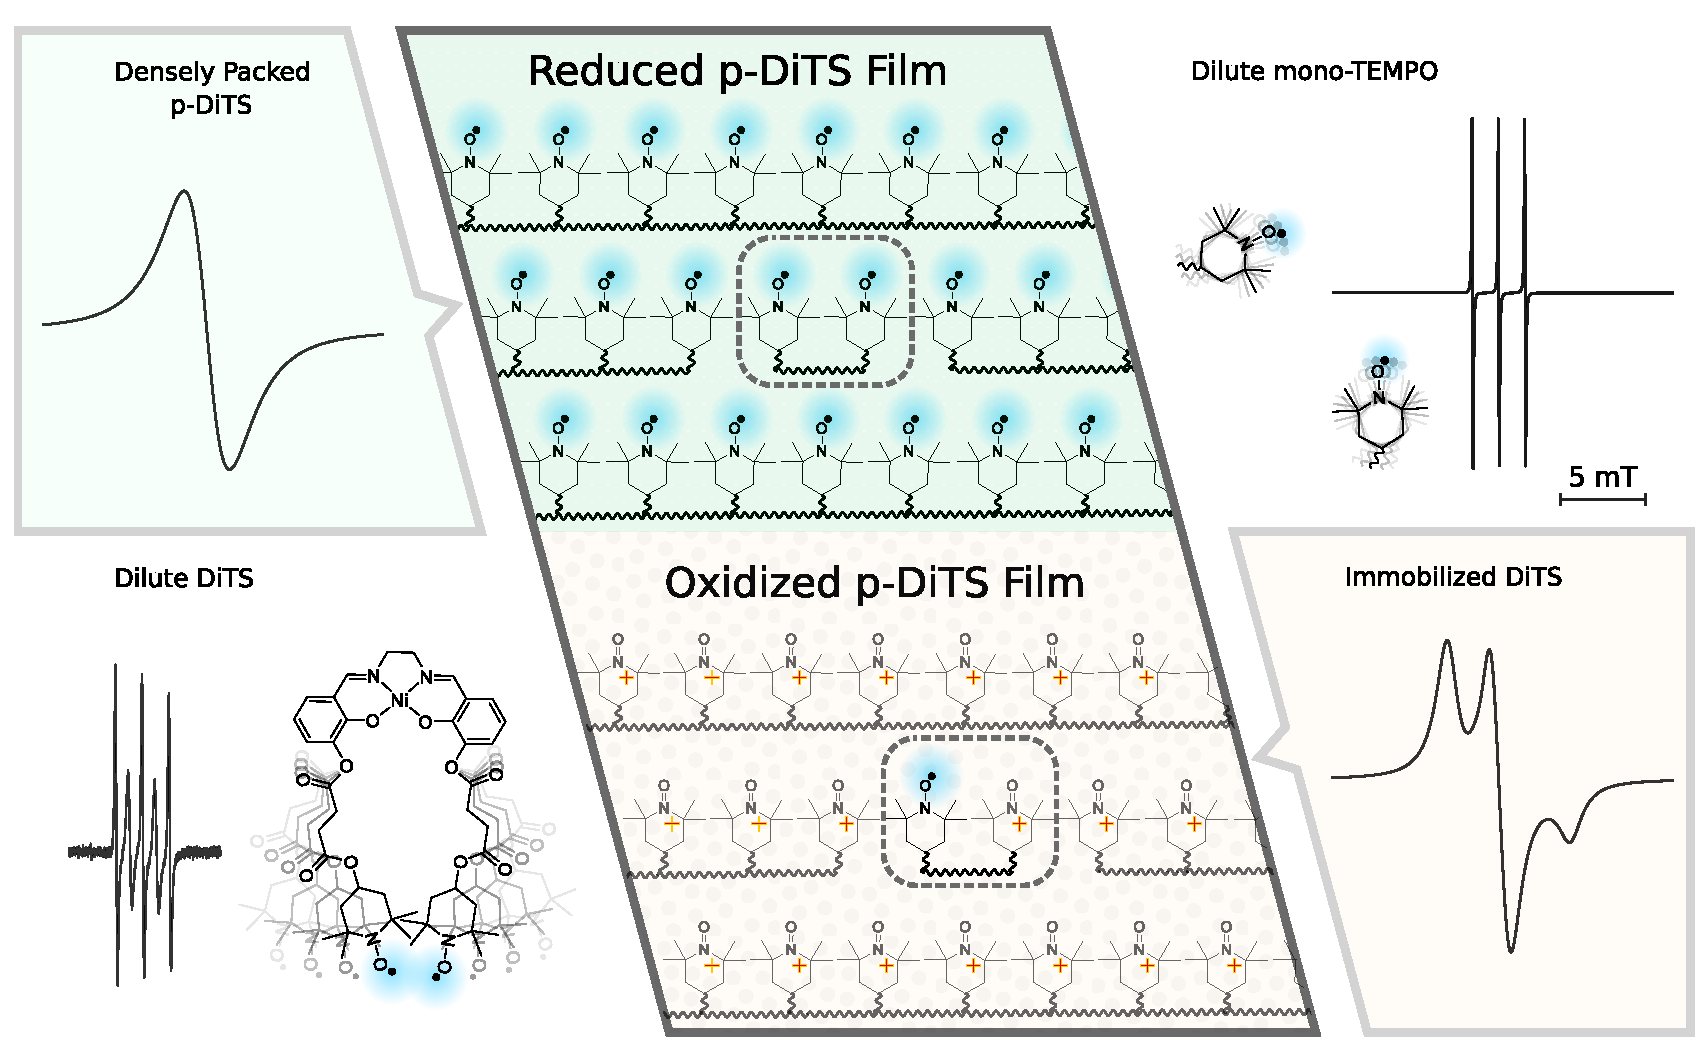
\includegraphics[width=1\textwidth]{./operando_epr/figures/Cartoon_ALL.pdf}
	\caption{Classification of the nitroxide cwEPR spectra observed for p-DiTS under different conditions and in different environments. a): Densely packed nitroxide film with dipolar broadening and exchange narrowing or broadening giving a single derivative line. b): Typical spectrum of dilute mono-nitroxide in solution, three-lines due to $S=1/2$, $I=1$ $^{14}$N hyperfine interaction (described by isotropic $g$-factor and isotropic hyperfine ($A$) interaction). c): Typical spectrum of tumbling di-nitroxide in solution where dynamic changes in the nitroxide -- nitroxide distance modulate the exchange interaction yielding a five-line structure with alternating line width (measured cwEPR of DiTS monomers in solution at room temperature). d): Immobilized nitroxide spectrum with both $g$ and $A$ anisotropy.}
	\label{fig:cartoon_spectra_dts}
\end{figure}


EPR spectra of electrochemical cells with p-DiTS as active-electrode material can exhibit a variety of different signals. Before presenting and discussing the experimental results, we will provide an overview about the various characteristic cwEPR lineshapes associated with nitroxides in different environments.
\par

Fig.~\ref{fig:cartoon_spectra_dts}a shows the spectrum expected for a \emph{densely packed p-DiTS film} with all nitroxides in the EPR-active reduced state. The broad unstructured line results from the strong dipolar and exchange interaction between both nitroxides of each DiTS monomer as well as between the nitroxides of different monomers. The exchange interaction can lead to either line narrowing or broadening depending on the strength of the interaction,\cite{Anderson1953} while the dipolar interaction causes broadening. In consequence, the overall cwEPR line width depends on the spin concentration in the film.
\par 
\emph{Dilute mono-TEMPO fragments} dissolved in the electrolyte, each containing only one nitroxide, give rise to a three-line spectrum (cf.\ Fig.~\ref{fig:cartoon_spectra_dts}b) which is well known from nitroxide-based spin labels in solution.\cite{Liu2008} Tumbling of the molecules in the liquid electrolyte results in an averaging of the anisotropic interaction between the electron spin and the nitrogen nuclear spin ($I = 1$) as well as of the $g$ anisotropy, leaving only the isotropic part of the hyperfine coupling and the isotropic $g$ value. 
\par
\emph{Dilute DiTS monomers} in the electrolyte generally give a spectrum consisting of five narrow lines (cf.\ Fig.~\ref{fig:cartoon_spectra_dts}c), if each monomer contains two interacting EPR-active nitroxides. The spectrum depends on dynamic effects, specifically the modulation of the exchange interaction between both radicals of each monomer.  Thus, depending on the solvent and temperature, the spectrum can be indistinguishable from the three-line spectrum of mono-TEMPO fragments.
\par
The fully charged (oxidized) p-DiTS film can contain electrically isolated domains in which the nitroxides are not connected to the electrode and cannot be oxidized or reduced. These electrically inactive \emph{immobilized DiTS monomers} in the oxidized film display a spectrum as shown in Fig.~\ref{fig:cartoon_spectra_dts}d. In contrast to the densely packed p-DiTS film, the dipolar and exchange interactions between neighboring radicals are much weaker. The anisotropy of the nitroxide's hyperfine tensor adds features to the cwEPR spectrum in d) as compared to a).
Yet, there is some remaining line broadening that does not allow one to distinguish between immobilized DiTS monomers with either one or two paramagnetic nitroxides.
\par
We note that the oxidized NiSalen backbone can contribute to the spectrum as well. Its EPR signature, which is not shown in Fig.~\ref{fig:cartoon_spectra_dts}, is clearly different from the nitroxide/TEMPO-related spectra discussed above.
%
























\subsection{Spectral Simulations}

\subsection{Quantitative Analysis of Potential-Dependent EPR Spectra}
\begin{figure}[h]
\center
	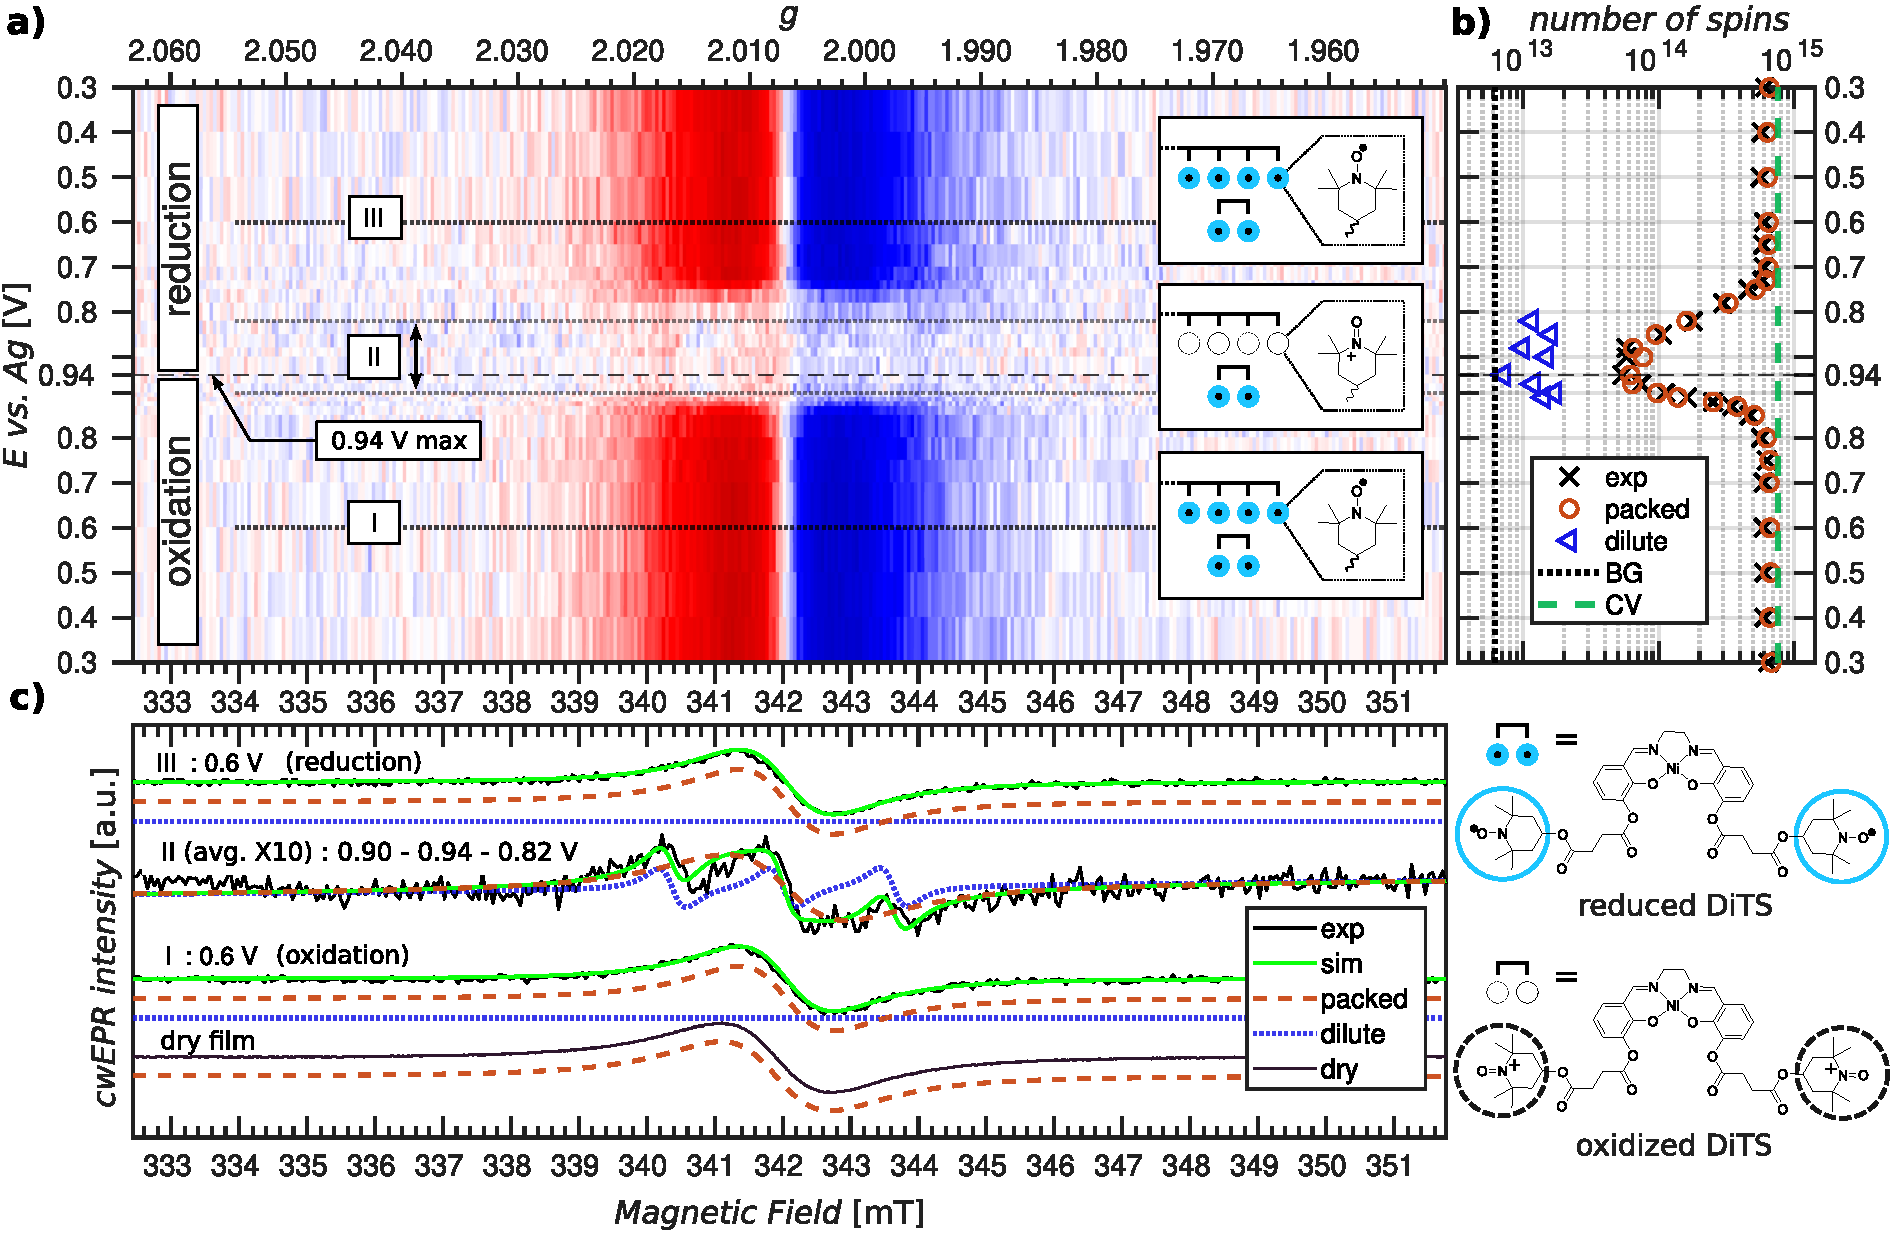
\includegraphics[width=1\textwidth]{./operando_epr/figures/Main_2D_redox_map_full.pdf}
	\caption{XXX}
	\label{fig:operando_carpet}
\end{figure}
\subsection{EPR-Detected State Of Charge}

\subsection{Formation of Singlet Spin States in a Reduced Cathode Film}

\subsection{Monitoring of Degradation Processes}
The operando monitoring of EPR spectra in pDiTS cells has revealed that the amount of paramagnetic species reduces upon the cycling. The cwEPR spectra during one charge-discharge cycle of two different pDiTS cells are shown in Figure~\ref{fig:operando_degradation}. Both datasets show a significant amount of the three-line structure in the oxidised (fully charged) state, that corresponds to the the release of dilute nitroxide radicals from the polymer film to the electrolyte. The fact that the released species exhibit a 3-line structure and not a 5-line structure excludes the release of the di-TEMPO (DiTS) monomers and suggests that individual TEMPO$^{\bullet}$ fragments are being detached from the film. Therefore, it was found that it is the molecular degradation of DiTS that is responsible for the loss of cell's capacity and not the decomposition of the polymer film into the monomer fragments. The overall EPR signal intensity decreases for both samples after the charge-discharge cycle. The spectral deconvolution with quantitative analysis of the individual components has revealed that the released fragments do not explain the overall loss of the signal intensity after the cycle.


\begin{figure}[!h]
\center
	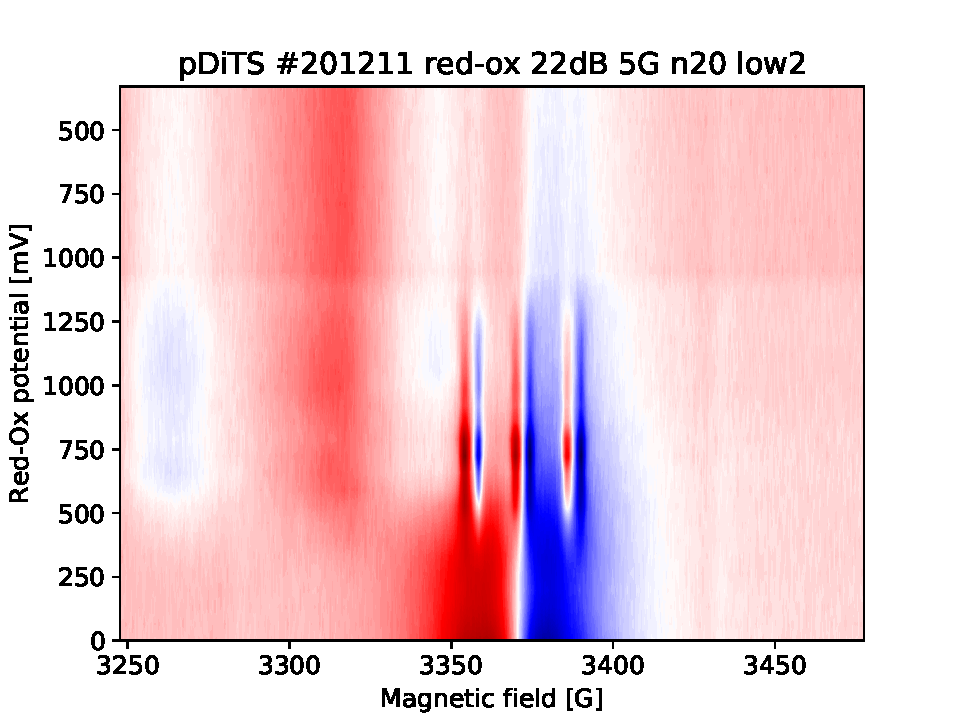
\includegraphics[width=1\textwidth]{./operando_epr/figures/degradation/overnight_dits_201211_full_redox_contour_XY.pdf}
	\caption{Operando cwEPR spectra of a pDiTS electrochemical cell showing irreversible release of charge-bearing fragments and decomposition of the device upon the extreme charging currents.}
	\label{fig:operando_degradation_device}
\end{figure}


\begin{figure}[!h]
\center
	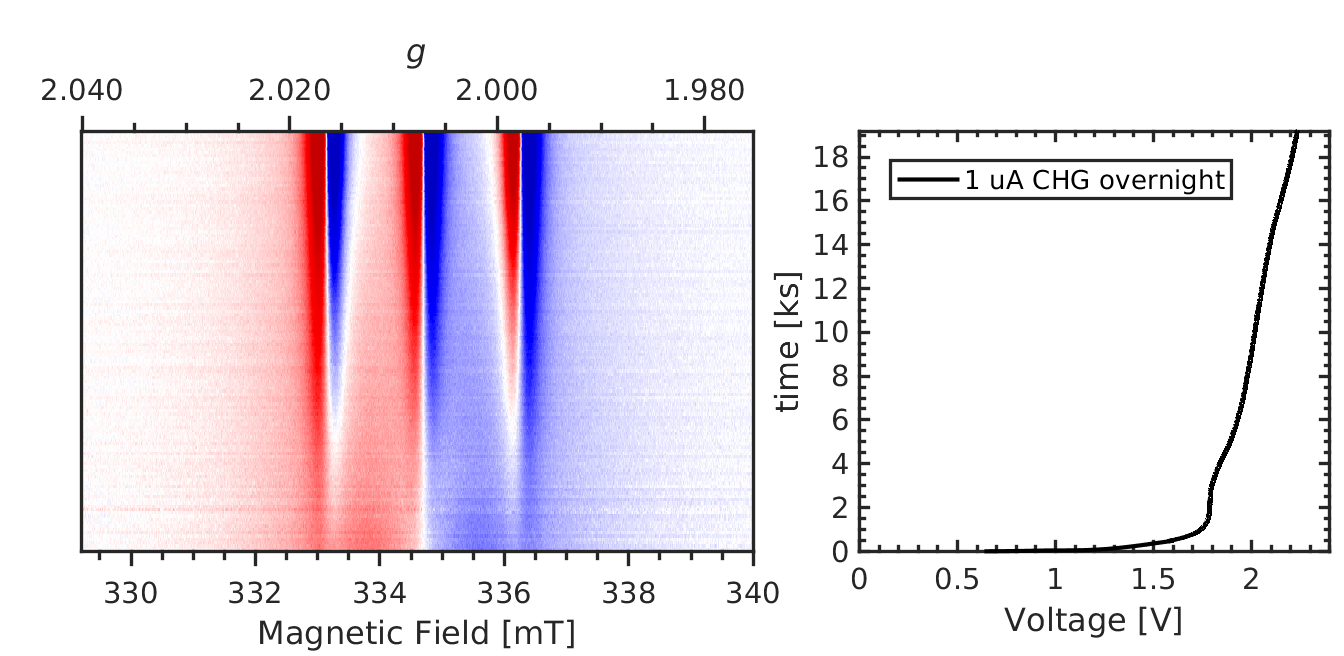
\includegraphics[width=1\textwidth]{./operando_epr/figures/degradation/pDiTS_slow_charge_MS5000_forslides.png}
	\caption{Operando cwEPR spectra of a pDiTS electrochemical cell showing irreversible release of charge-bearing fragments upon moderate charging currents.}
	\label{fig:operando_degradation_3_lines_release}
\end{figure}


\begin{figure}[!h]
\center
	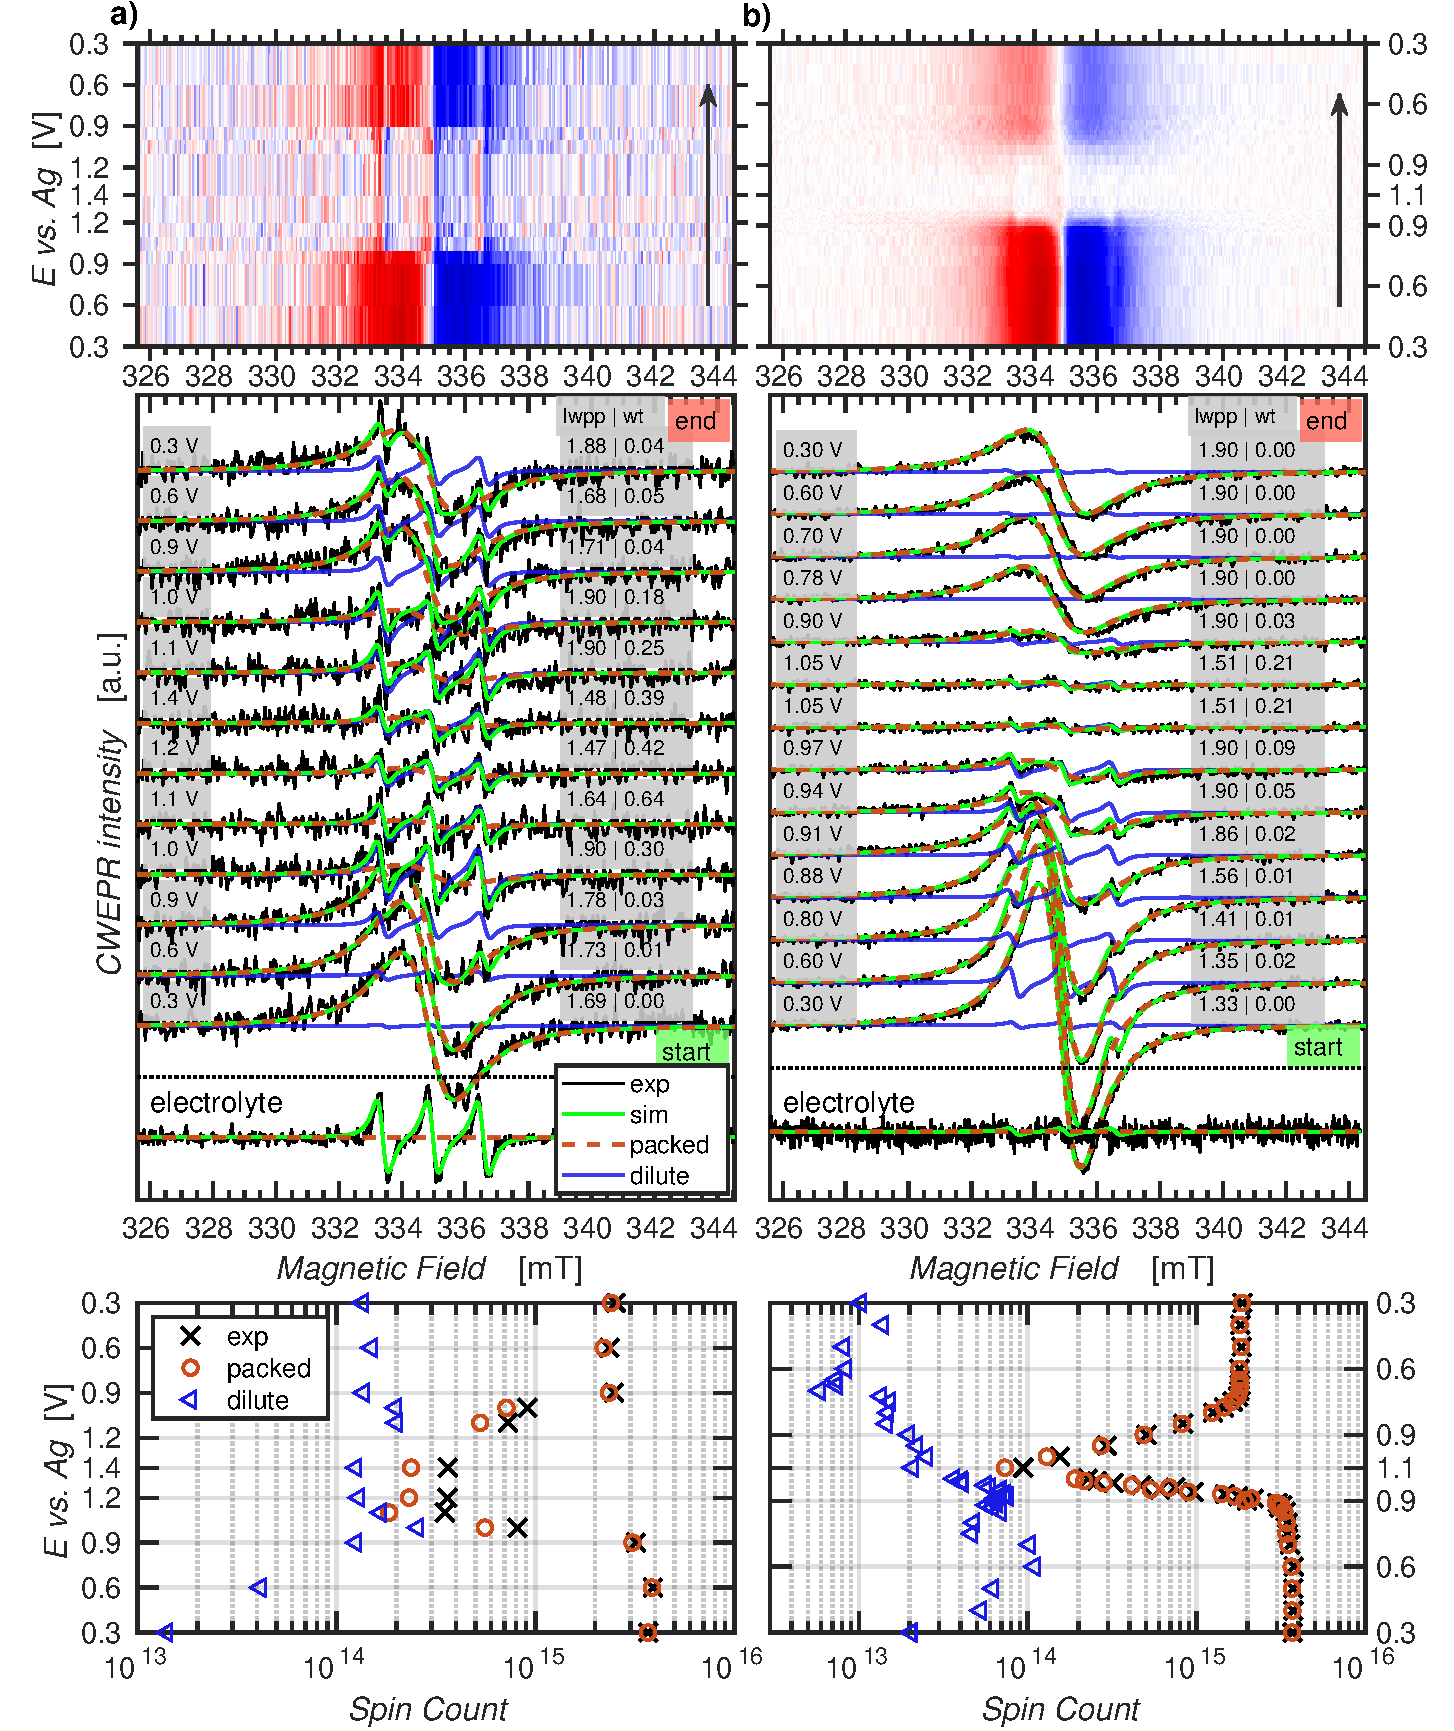
\includegraphics[width=1\textwidth]{./operando_epr/figures/degradation/operando_degradation_dits.pdf}
	\caption{Operando cwEPR spectra of two pDiTS electrochemical cells showing release of charge-bearing fragments upon the charge-discharge cycle.}
	\label{fig:operando_degradation}
\end{figure}

\begin{figure}[!h]
\center
	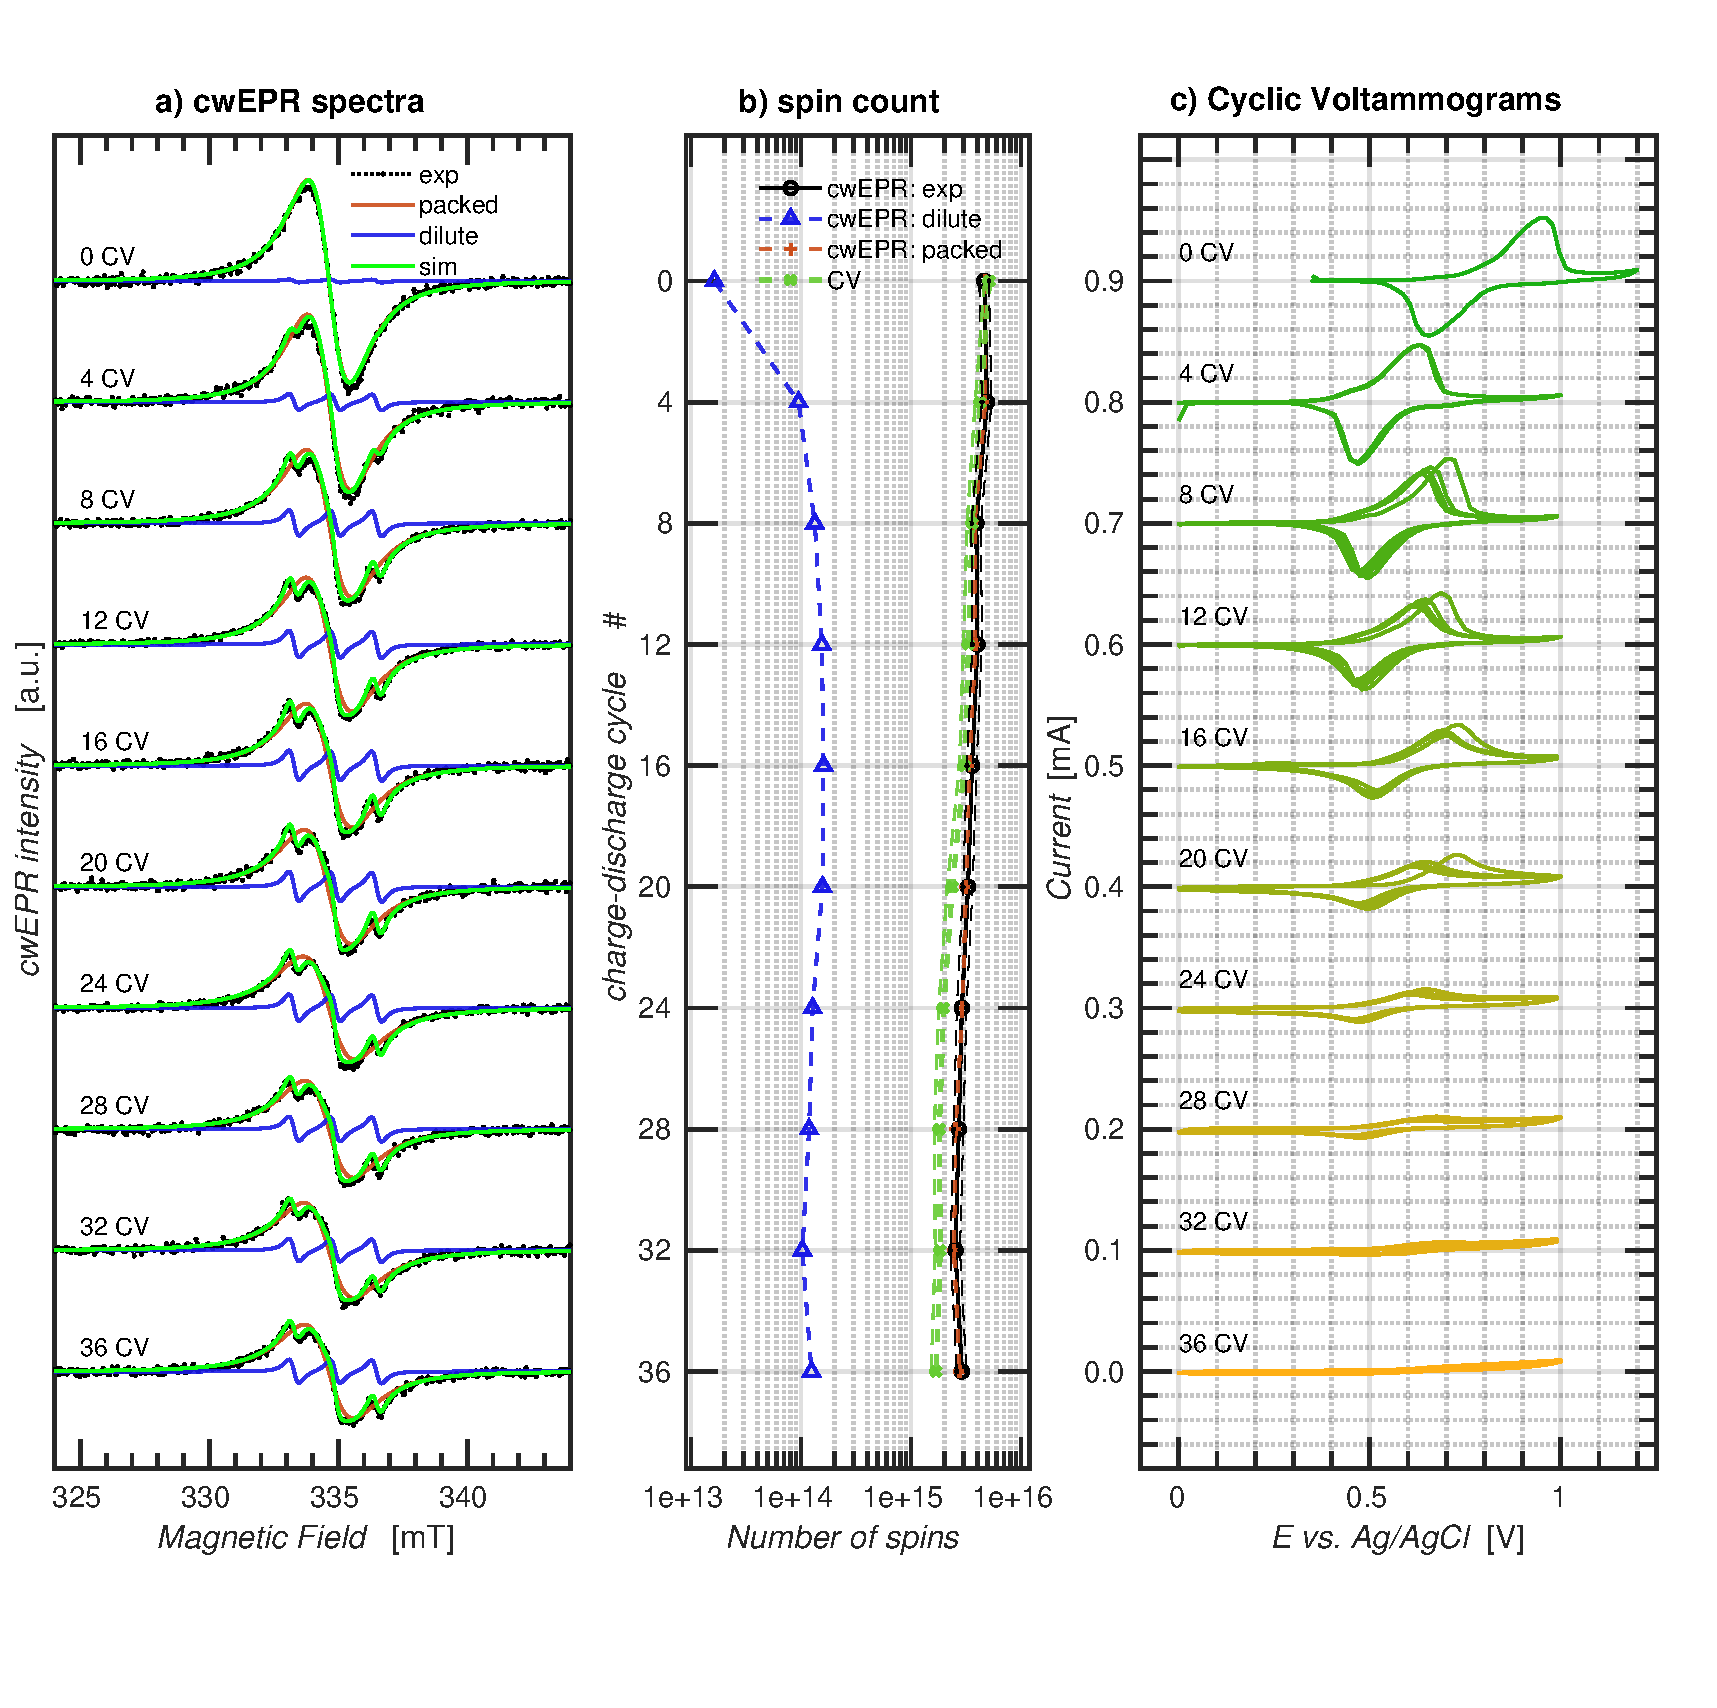
\includegraphics[width=1\textwidth]{./operando_epr/figures/degradation/repeated_cycling_degradation_dits.pdf}
	\caption{ZZZ}
	\label{fig:repeated_cycling_degradation}
\end{figure}





\subsection{Monitoring of Self Discharge}
Organic Radical Batteries have a tendency to self-discharge, as the organic electrochemically active layer partially dissolves in polar electrolytes. Particularly for the TEMPO containing ORB, the dissolved, mobile TEMPO fragments serve as redox shuttles that carry the charge between the battery electrodes and cause a self discharge. The amount of unoxidized TEMPO$^\bullet$ shuttles can be measured with cwEPR spectroscopy as the mobile fragments have distinct spectra as compared to the fragments tightly packed in the electrode. Further in this subsection operando spectra of a TEMPO containing electrochemical cells are shown. Quantitative analysis of the released fragments during a charge-discharge cycle allows for a description of the self-discharge process in an ORB. The charge state of a battery is monitored with cwEPR and, additionally, with a potentiometric measurement to identify the self-discharge rate and to connect it with the concentration of diffusing redox shuttles.

\subsection{Electrochemical Cells with Solid Electrolyte}





\subsection{Low Temperature Measurements}
\begin{figure}[h]
\center
	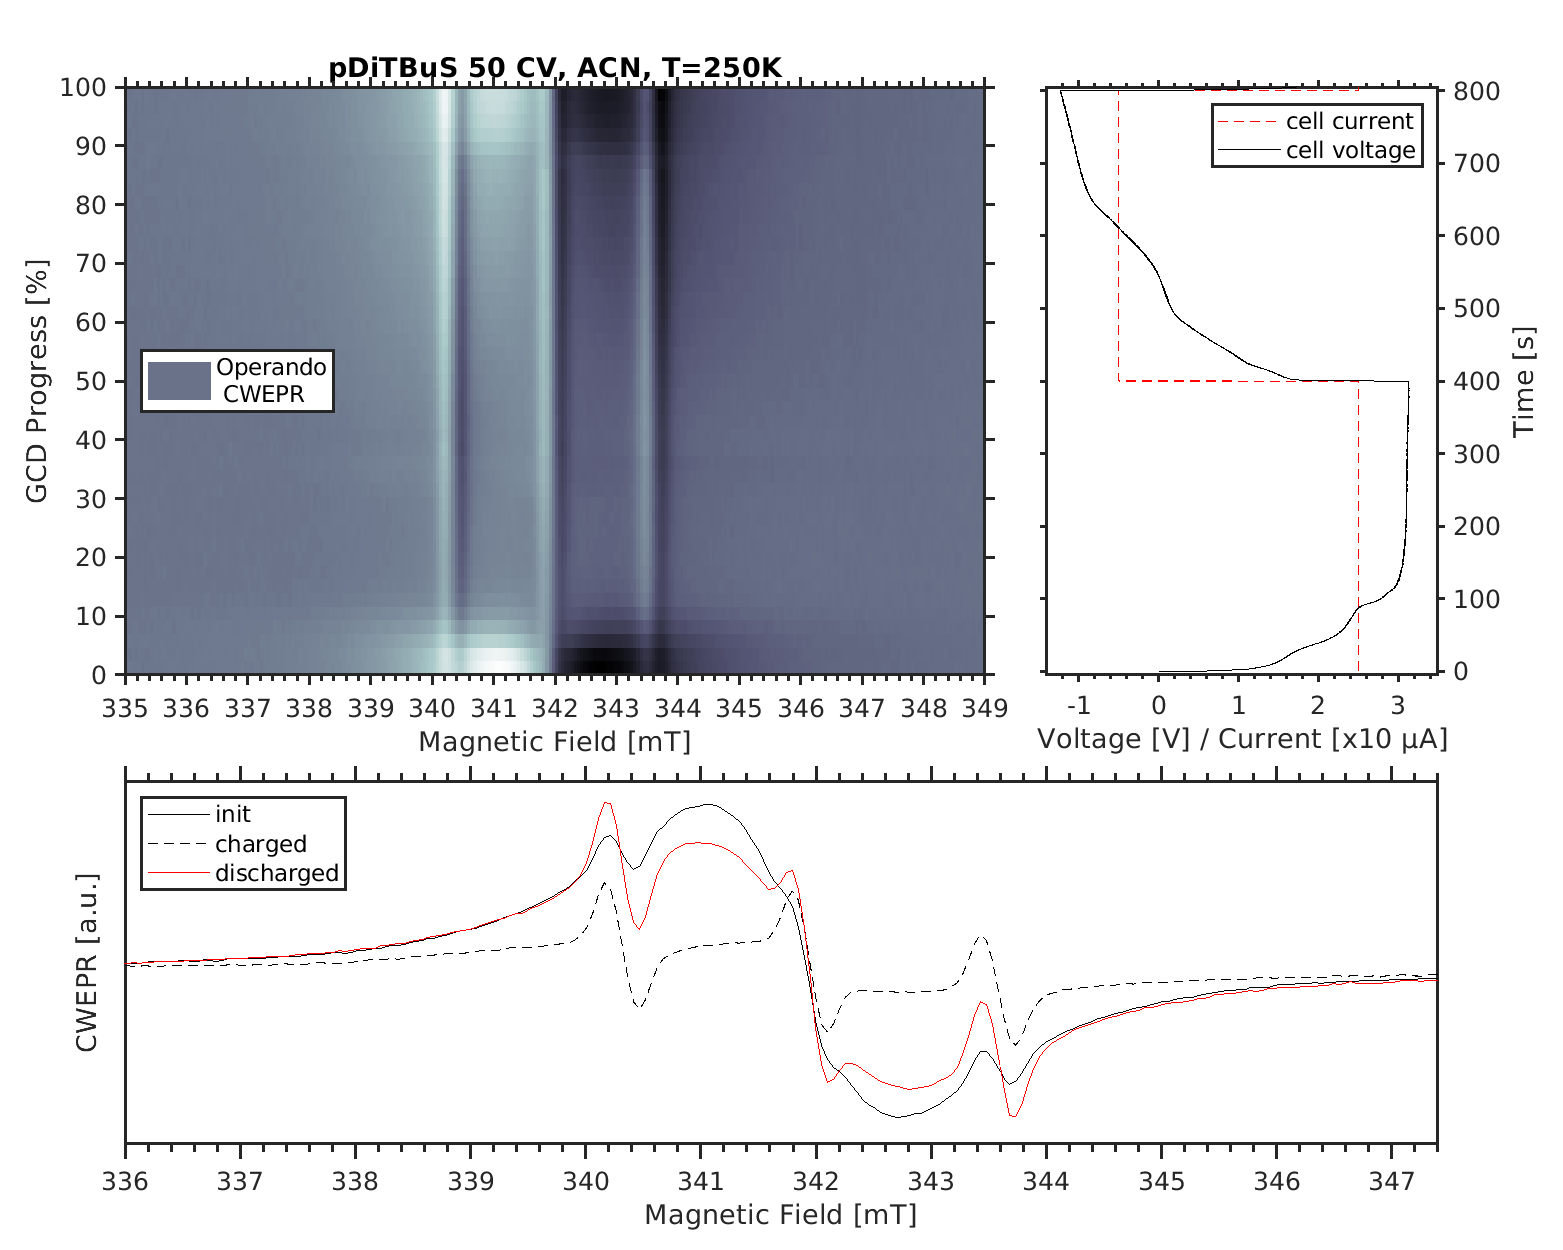
\includegraphics[width=1\textwidth]{./operando_epr/figures/slowcharge_231117_liquid_250K.pdf}
	\caption{XXX}
	\label{fig:operando_cold_cycle}
\end{figure}

